\documentclass[11pt]{report}

\usepackage[pdftex, xdvi, dvips]{graphicx}
\usepackage{amssymb}
\usepackage{doublespace}
%\usepackage{epstopdf}
%\DeclareGraphicsRule{.tif}{png}{.png}{`convert #1 `basename #1 .tif`.png}


%\usepackage{amsmath}


\textwidth = 6.5 in
\textheight = 9 in
\oddsidemargin = 0.0 in
\evensidemargin = 0.0 in
\topmargin = 0.0 in
\headheight = 0.0 in
\headsep = 0.0 in
\parskip = 0.2in
\parindent = 0.0in



\newtheorem{theorem}{Theorem}
\newtheorem{acknowledgement}[theorem]{Acknowledgement}
\newtheorem{algorithm}[theorem]{Algorithm}
\newtheorem{axiom}[theorem]{Axiom}
\newtheorem{case}[theorem]{Case}
\newtheorem{claim}[theorem]{Claim}
\newtheorem{conclusion}[theorem]{Conclusion}
\newtheorem{condition}[theorem]{Condition}
\newtheorem{conjecture}[theorem]{Conjecture}
\newtheorem{corollary}[theorem]{Corollary}
\newtheorem{criterion}[theorem]{Criterion}
\newtheorem{definition}[theorem]{Definition}
\newtheorem{example}[theorem]{Example}
\newtheorem{exercise}[theorem]{Exercise}
\newtheorem{lemma}[theorem]{Lemma}
\newtheorem{notation}[theorem]{Notation}
\newtheorem{problem}[theorem]{Problem}
\newtheorem{proposition}[theorem]{Proposition}
\newtheorem{remark}[theorem]{Remark}
\newtheorem{solution}[theorem]{Solution}
\newtheorem{summary}[theorem]{Summary}
\newenvironment{proof}[1][Proof]{\textbf{#1.} }{\ \rule{0.5em}{0.5em}}
%\input{tcilatex}


\title{Matrix Multiplication, Inversion and Partial Differential Equations via Wavelets}
\author{Daniel Beatty}

\begin{document}


\maketitle \newpage

\tableofcontents \newpage

\chapter{Introduction}
Some overwhelming questions that drive computational science are how
fast can the answer be computed, how accurate is the answer, and how
stable is the method for obtaining the answer.  In this thesis, these
questions are applied to matrix multiplication. Of course there are already
conventional algorithms to compute matrix multiplication. This thesis
contributes a simple analysis of how the wavelet operator can be applied
to matrix multiplication.

The two most desired qualities in the computation of matrices are
sparseness and the condition number. Sparseness for a matrix states
that a good majority of the elements in such a matrix are zero.  The
condition number indicates how accurately an operation will be
performed on the system.  Wavelets contribute to numerical methods by
providing a stable preconditioning technique which produces a more
sparse and better conditioned than the original matrix.  Various forms
of the wavelet transform are key to applying wavelets as a
preconditioning tool.

Matrix multiplication has applications in simulations, computer
vision, and almost all areas of computational science.  Classic matrix
multiplication has a computational complexity of order $N^3$
operation, which makes it costly in the number of instructions that
are needed to carry out the operation. Faster matrix multiplication
techniques depend on the matrix being sparse to reduce the number
elements that need to be multiplied.  As shown in the results section,
there exists various levels of acceptable sparseness that are
generated by the wavelet transform.

For matrix multiplication, wavelets provide a preconditioning method
that transforms a dense matrix into a sparse one.  Thus sparse matrix
multiplication can be applied more effectively to general class of
matrices.  Wavelet preconditioning may or may not help for matrices
that are already sparse.

In this thesis, an overview is provided to define wavelets and how to
apply them.  This overview uses image processing to demonstrate the
qualities of a two-dimensional wavelet transform.  The next chapter
describes the wavelet matrix multiplication procedure. Chapter
\ref{chp:results} demonstrates matrix multiplication in the wavelet
domain and shows the results of different threshold levels on the
fidelity of the resulting product.  Finally, conclusions are
presented.



\chapter {Overview on Wavelets}
Goals for this introductory document on wavelets is to define a wavelet,
acknowledge alternative definitions of a wavelet, specify basic wavelet
theorems, and show wavelets through practical examples. \ \ Convolution provides the key for defining the wavelet, its theorems and practical examples.  The Haar Wavelet Filter is used to show these concepts.  

\section{Wavelet Transform Definitions}

As stated, the wavelet transform can be viewed from both a matrix
representation\cite{matrix01} and vector convolution. Both
representations provide means to use many linear algebra and abstract
algebra methods to prove theorems about wavelets.  Another form is a
convolution type of operation. Convolution wavelet transform methods
provide a simple computational method in general. Special case
convolution methods also exist, which allow even simpler algorithms to
perform wavelet transforms.

In the matrix form, a wavelet matrix is defined as a generalization of
a square orthogonal or unitary matrix which is a subset of a larger
class of rectangular matrices . This matrix harvests information for
defining a wavelet system.  Such matrices are defined in terms of
their rank and genus\cite{matrix01}.

It was Alfred Haar himself who defined an orthonormal wavelet matrix
in ``Zur Theorie der orthogonalen Funktionensystem Math Annual''
written in 1903. The said wavelet was named in honor of Alfred Haar,
the Haar Wavelet Matrix. A Haar Wavelet Matrix has a genus of
one. Such matrices have a one to one mapping to a general wavelet
matrix. Also, Haar Wavelet Matrices are equivalent to the
characteristic Haar Matrix. Lastly, a rank 2 Haar Matrix embodies all
geometric considerations\cite{matrix01}.

\section{Wavelets via Convolution}

Wavelets are defined in terms of average and difference components.
Each component can further be transformed to isolate properties of
each component.  Typically, each component has the form $S\rightarrow
(A|D)$ where $S$ is the original signal, $A$ is the average component, $D$
is the difference component and $(A|D)$ the signal $A$ concatenated with
$D$.  Each of these components are produced by an orthonormal basis.
Also, these components are produced such that the original can be
constructed easily from them.

Many mathematicians such as Walker\cite{walker}, use a form that
eliminates half of the values. Thus a form can be defined which has
the same number of elements as the original.  The rules for choosing
the member elements are dependent on the wavelet filter choice.


Another useful property of wavelets via convolution is the simplicity
of the operation. The general case works for all.  Such an algorithm
requires one nested loop as seen below:

\begin{tt}
\begin{tabbing}
$\forall i\in \lbrack 0,M)$ \\
\qquad $\forall j\in \lbrack 0,N)$ \\
\qquad \qquad n=i-j \\
\qquad \qquad if ($n\in \lbrack 0,M)$) \\
\qquad \qquad \qquad $y_{i\,}+=x_{n}\cdot h_{j\,}$
\end{tabbing}
\end{tt}

This filter simply equates to the mathematical function: $x\ast
h=\sum_{l}h(l)x(k-l)$, which is the convolution operation. As we can
see the operation is slightly less than $O(N^{2})$ . For practical
use, the filter is made smaller than the actual signal being
analyzed. In some cases, the filter may be much smalled than the
signal. Filter size matters in extracting features from the original
signal.

In the case of this convolution operator, the limit is actually $M$, not
$N$.  The value of $M$ is the size of the original signal. Since the
resulting vector is the same as the original, the vector is said to be
fully qualified. Only half of those values are necessary to
reconstruct the original (every other element).

To perform a wavelet transform via convolution, each signal is
convolved twice.
\[
A_{i}=A_{i-1}\ast V,
\qquad \qquad
D_{i\,}=A_{i-1}\ast W
\]
where 
\begin{itemize}
\item $V$ is the scaling wavelet vector,
\item $W$ is the differencing wavelet vector,
\item $A$ is the average vector (scaled vector),
\item $D$ is the difference component vector,
\item $\forall i\in \lbrack 1,L)$ and $A_{0}=f$ which is the
original signal, and
\item $L$ is the limit on the number resolutions that signal can have
based on the wavelet type.
\end{itemize}

\section{Class 2D Wavelet: Complete Form}

The convolution version can be used to derive a Wavelet Matrix.  For a
general case, it is simpler to use the convolution method.  The matrix
form becomes practical in repetitive special case applications.

The 2D transform has four components: the average, vertical,
horizontal, and diagonal. Two general computational means exist to
generate a one-resolution transform.  These can derive means for
performing many resolutions.

A complete transform method returns a result matrix which is the same
size as the source matrix. The result contains the four
components. Each component resides on 4 corners of the matrix. Given a
matrix $B$, the transform is to yield the following form:
\[ 
B \Rightarrow 
\left(
\begin{array}{cc}
H & D \\ 
A & V
\end{array}
\right)
\]
where $A$ is the average component, $H$ is the horizontal component,
$V$ is the vertical component, and $D$ is the difference
component. There is another form which is also used as an example:
\[
B \Rightarrow 
\left(
\begin{array}{cc}
A & V \\ 
H & D
\end{array}
\right)
\]
The first version is simple in concept, but provides a few more
possibilities for error and confusion.  Regardless of the case, the
four components have the following definitions:
\begin{enumerate}
\item Average component: produced by filtering the row vectors and the column vectors with the averaging filter.
\item Vertical Component:  produced by applying the average filter to the column vectors and the difference filter to the row vectors.
\item Horizontal component: produced by applying the average filter to the row vectors and the difference to the column vectors.
\item Diagonal component: produced by applying the difference filter to both the row and column vectors.  
\end{enumerate}

\subsection{Proof of Concept}
Two methods of convolving a matrix are easily conceived.  First is to
use 1D wavelet.  The other is to apply the convolution scheme
straight to the matrix. Included in the wavelet experiment are both.
Realistically, both can and do achieve the same result.  However, the
direct method achieves speed advantages by the lack of overhead.  The
direct method only stores a temporary vector resident in memory.  Also,
there are two fewer transfers per row and column.

\subsubsection{1D to 2D Method}

Both rows 1D and 2D and columns 1D and 2D transform are performed
similarly.  The obvious difference is the indexing of rows and
columns.

Given: 1D wavelet transform
source matrix

Algorithm: (Row Transform)

$\forall i \in rows$
\begin{itemize}
	\item $\forall j \in columns$
	
	\item $S[j] \leftarrow source[i][j] $
	
	\item $S \Rightarrow ^W  R$
\end{itemize}

This principle of this algorithm is simple.  Only three intuitive steps are necessary per row or column.  Two of these steps are array transfers (row/column transfer to an array).  These arrays are fed into the 1D transforms.  

However, the 1D wavelet transform itself includes a series of memory allocation and deallocation operations.  Each memory call is at the minimum a system call.  

\subsubsection {Vector - Matrix Method}
The principle of this algorithm is more complicated.  All functionality, such as convolution, is built into the method.  There are fewer calls and passing of structures to external functions to compute the transform.  

This method has a few givens.  The source matrix, the Haar average filter, and the Haar difference filter are given arguments.  The result argument is the return argument.    The transform signals sub-function row transforms and column transforms to perform the work.  

The algorithm is as follows for the row transform (and is similar for the column transform):  

$\forall i \in rows$
\begin{enumerate}
\item Initialize temporary array/vector to all zeros ($x$).
\item $\forall k \in columns $
\begin{enumerate}
\item $\forall l \in ha.Size$
%$
%x += 
%\begin{cases}
%S_{i,k-l} \ast hA_l, & \text{if $k-l \in columns$} \\ 
%0, & \text{otherwise}
%\end{cases}
%$

\end{enumerate}
\item $\forall k \in columns/2 $

$result_{i,k} = x_{2k+1} $  (In other words, odd split)

\item Initialize $x$ to all zeros.
\item $\forall k \in columns $
\begin{enumerate}
\item $\forall l \in hd.Size $

%$
%x +=$  
%\begin{cases}
%$S_{i,k-l} \ast hD_l$, & \text{if $k-l \in columns$} \\ 
%0, & \text{otherwise}
%\end{cases}


\end{enumerate}


\item $\forall k \in columns/2 $

$result_{i,k+columns/2} = x_{2k+1} $  (In other words, odd split)


\end{enumerate}

\subsection {Multiresolution}

The multiresolution wavelet transform and the inverse multiresolution transform resemble the vector-matrix version.  All functionality is built into this method.  However, there are structural changes.

The wavelet transform (multiresolution) uses private members of the class ($hA$, $hD$, $xD/yD$, $xA/yA$).  Both Haar filters are maintained this way.  Also both row and column transforms have average and difference myVector classes for temporary storage.   All of these members are allocated and destroyed by the wavelet transform method itself.   The simplified algorithm of the row transform is the following:
\begin{enumerate}
\item Initialize $xA$ and $xD$ to zero
\item $\forall k \in columns, \qquad \forall l \in filter$
\begin{itemize}
\item $n = k - l$
\item if ( $n \in columns $ )

	$xA_k = W_{i,n} * hA_l $
	
	$xD_k = W_{i,n} * hD_l $
	
	
\end{itemize}
\item Transfer back to W

	$W_i = xA|xD $
\end{enumerate}

And the column transform is represented by:
\begin{enumerate}
\item initialize $yA$ and $yD$ to zero
\item $\forall k \in rows, \qquad  \forall l \in filter$
\begin{itemize}
\item $n = k - l$
\item if ( $n \in columns $ )

	$yA_k = W_{i,n} * hA_l $
	
	$yD_k = W_{i,n} * hD_l $
	
	
\end{itemize}
\item Transfer back to $W$

	$W_j = yA|yD $
\end{enumerate}

Note: $W_i$ names the row vectors and $W_j$ names the column vectors, and $W_{i,j}$ is the element from the $i^{th}$ row and $j^{th}$ column.


%\subsection {Wavelet Transform: Quad Tree}
% The primary two addition to the wavelet transform in case of the Quad Tree variety is the tree and spare matrix.  The spare matrix is used to keep the transform operation separate during computation.  This may not be necessary in distributed versions.  

%The quad tree node has 9 elements side from links to 
%\begin {itemize}
%\item Energy (the section energy)
%\item coordinates for the upper left corner
%\item coordinates for the lower left corner
%\item coordinates for the upper right corner
%\item coordinates for the lower right corner 
%\end{itemize}

%The procedure for the quad tree wavelet transform involves loading the root node with its coordinates and the energy of the matrix.   This energy is used as an early stopping condition.  In the non-distributed form, it useful to load a temporary matrix global to the class/ object for the purpose of memory conservation, and system call conservation.  

%Given quad tree node, The steps are to compute the column wavelet transform followed by the row transform on matrix one and matrix two.  Following the computation of the wavelet transform, the energy for each segment must be computed.  If the energy limit (epsilon) or size limit has been reached, then stop procedure must be initiated.  Otherwise, the computation is continued for the 4 sub-components produced by the current wavelet transform.  

% The quad tree requires another feature in its structure, breadth first and depth first searching.  The purpose behind these searches is to extract the structure of the wavelet quad-tree transform and store it in an array.  This array can then be stored in a database, file, or passed to another procedure or returned to a calling procedure.  In the case of the leaves, this array can be made to store the actual matrix data, and its dimensions in another array.  

% The breadth first search requires a queue structure to hold pointers to the tree nodes.  First the root is put queue.  While the queue is not empty, the bread first search works on elements in the queue in a loop.  

% First step in the loop is to pop the element in the queue. Then stores that information.  Next the four children are inserted into the queue.  Then loop is repeated.  The only time that elements are not added to the queue is if they themselves are empty.  Eventually, the leaves are all reached, which have empty children.  This cause the queue to exhaust itself, and terminate the loop.  

% The depth first search essentially uses a stack, which implies that a recursive method can also be used.  The visit procedure is as follows:

% In particular there are two places where these traversal methods are necessary for the search, store, retrieval, transform, and inverse transform.  The first three are somewhat obvious.  The transform and inverse transform are not trivial.  

% In the depth first method, the transform is performed first for the average branches, starting at the root.  Once the average branch is transformed, the vertical branch is transformed by treating the first vertical child as its own root, and recursively repeating the transform.  This is again done for the horizontal and diagonal components.  

% The breadth first method first transforms the root, the same as the other methods.  Next, the branches formed by the transform are placed into a queue, and those elements are then transformed.  The step is repeated for subsequent transforms of each branch.  

% A hybrid approach takes the four branches after the transform uses size to evaluate whether to breadth first or depth first.  In the case of depth first, all four branches performed by separate threads of execution since the operations are independent of one another.  

% \subsubsection {Tree - Queue representation.  }
% For efficiency in speed, this implementation uses an array based tree and queue.  The reason is for ease of traversal, copying, storing, and retrieving.  The relation on the the array is as follows:
% \begin{itemize}
% \item $i_r = \frac{i_c -1}{4}$
% \item $ i_a = 4 i_r + 1$
% \item $ i_a = 4 i_r + 2$
% \item $ i_a = 4 i_r + 3$
% \item $ i_d = 4 i_r + 4$
% \end {itemize}

% Second is the construction of the tree data being stored.  For these experiments, wave-node keeps the energy of the matrix, the maximum value, the minimum value, the four corners, width, and width.

\subsection {Computational Cost}
The cost of this algorithm is computed first for each row and each column.  This value is used to compute the cost of the matrix. The cost of computing the matrix is used to compute the cost of the multiresolution steps.   Per row the cost is $3K$, where $K$ is the number of columns.  Per column the cost is $3L$, where $L$ is the number of rows.  For the whole matrix, one resolution costs $6KL$ operations to compute the wavelet transform.    Per resolution, the rows and columns shrink by $2^i $ for each resolution, i, performed.  The limit of this cost equals $12KL$ operations.  Thus, the cost is linear.  

%Stopped at this point April 10, 2003
\section{Results - 1D Wavelet Transform}
Testing of the 1D wavelet was performed on a sinusoidal wave form of 128 elements.  The given function has the equation shown in Figure \ref{sample}.

\[
y(n) = 10 \sin \left({n \over 128}\right) 
	- 5 \sin \left({n \over 64}\right) 
	+ 2 \sin \left({3 n \over 128}\right)
	- \sin \left({n \over 32}\right)
\]

\begin{figure}
\includegraphics [width=4in]{sample.jpg}
\caption{Sample function.  The $x$-axis is the array index (index $n$).  The $y$ value is simple -- the value $y(n)$. }
\label{sample}
\end{figure}


The first version of the 1D transform used the even elements of both convolutions to generate the wavelet transform.  These even elements came from the over-complete form and naturally allow the potential to have complete information.  However, in doing so, a fundamental flaw appears.

In order to evaluate the effectiveness of the wavelet transform three tests have been devised.  First,  energy equivalence is used to determine how much energy is retained in the transform from the original.    The general shape is used on a the first resolution to test if the average signal has the same general shape as the original.  Lastly, the inverse transform is used to recover the original signal.  A comparison is made between the original and the recovered signal.  

After one resolution, the transformed signal has the same energy as the original.  This is good since it allows the original to be recovered from the transform.  Also, the average component of the transform has the same shape as the original.  This is good.  However, the recovered signal is missing the last element.  Refer to Figure \ref{recoverEven}. The secret is in which elements are used from the over-complete to make the complete.  The over-complete in this project comes from the average component and difference which are simply the result of convolution.  

The convolution means is at the heart of the issue.  The convolution operator in this case starts with the first element of the filter against the first element of the signal.  In the simple Haar Wavelet case, there is a transformation pairing
\[
(S_i , S_{i-1}) \rightarrow A_i, \mbox{ and } (S_i , S_{i-1}) \rightarrow D_i .
\]
In this pairing with zero indexed signals, the odd indexed elements from the over-complete must be used to have all elements of the original accounted for.   

Also this produces a functional difference between wavelet inverse transform for odd and even versions.  The difference is slight; however, the last element is lost in the even indexed form.  

\begin{eqnarray*}
\mbox{Odd: } \qquad R_{2i} =(A_i - D_i ) \sqrt{1/2}, &\qquad& R_{2i+1}=(A_i + D_i ) \sqrt{1/2} \\
\mbox{Even: } \qquad R_{2i} =(A_i + D_i ) \sqrt{1/2}, &\qquad& R_{2i-1}=(A_i - D_i ) \sqrt{1/2} 
\end{eqnarray*}


%The even split  and analysis of this transform.  
\begin{figure}
\includegraphics [width=4in]{sample.jpg}
\caption{Recovered function.  The $x$-axis is the array index (index n).  The $y$ value is simply the value $y(n)$.  The function was recovered from an even indexed wavelet transform. }
\label{recoverEven}
\end{figure}

 
\begin{figure}
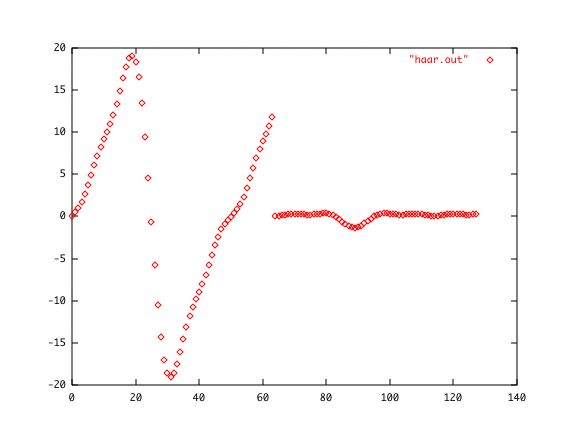
\includegraphics [width=4in]{recovered.jpg}
\caption{Recovered function.  The x-axis is the array index (index n).  The y value is simply the value y[n].  The function was recovered from an odd indexed wavelet transform. }
\label{recoverOdd}
\end{figure}

An odd indexed wavelet transform yields the same energy.  However, all of the values are accounted for.  Refer to Figure \ref{recoverOdd}.  

\section {Results: 2D Wavelet Transform }

A simple room picture shows the difference correct indexing produces in the wavelet transform and its inverse. The 1D to 2D method shows the incorrectly indexed case.  A correctly indexed version is shown in the vector-matrix method.  

The 1D to 2D method has a serious issue with memory leak errors (Macintosh OSX, using gcc 3.1).  Memory is allocated and deallocated quickly, and on some platforms shows up as an error.   On other platforms, the result is degraded performance (IRIX, SGI Octane2 using gcc 2.9).   An example image of 720 x 486 requires nearly 10 minutes to compute the wavelet transform by this method on an SGI Octane2.  However, this method does eventually return a correct result.  

The matrix-vector method also yields the correct result.  However, there is less memory overhead in this method as compared to the 1D to 2D method.  As a result, both the row wavelet transform and column wavelet transforms are performed more quickly, with fewer memory transfers and allocations.  Obviously, this also allows for the operation to be conducted almost entirely in cache memory on both the SGI Octane2 and Macintosh G4 based machines.  A Macintosh G3 based machine still requires main memory at a minimum to execute the same operation which yields a slower performance.  

A correct result must also be matched to a correct inverse method.  The indexing order matters.  The inverse transform method is a forward inverse transform method.  In the case of 1D to 2D transform, the ordering was reverse indexed (Figure \ref{rightWavepic}).  As a result of an error in indexing, ringing is seen on edges in this method(Figure \ref{rightDanRecovered}) for a case in point.  Caution is incredibly important when matching both forward and reverse indexing, since matching the mathematics to the actual ordering can be obscure and tricky.   

A correct result is shown in Figure \ref{selfRecover}.  In this case, the indexing was matched up and ringing is not present.  It is clear that the recovered image and the original (Figure \ref{rightDan}) are nearly indistinguishable.  

\begin{figure}[htb]
\begin{center}
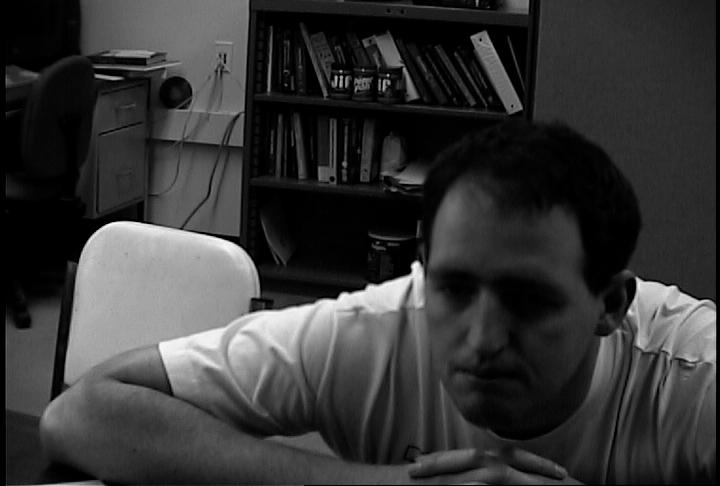
\includegraphics [width=4in]{rightDan.jpg}
\end{center}
\caption{Original Image.  This image is the original image. }
\label{rightDan}
\end{figure}

\begin{figure}[htb]
\begin{center}
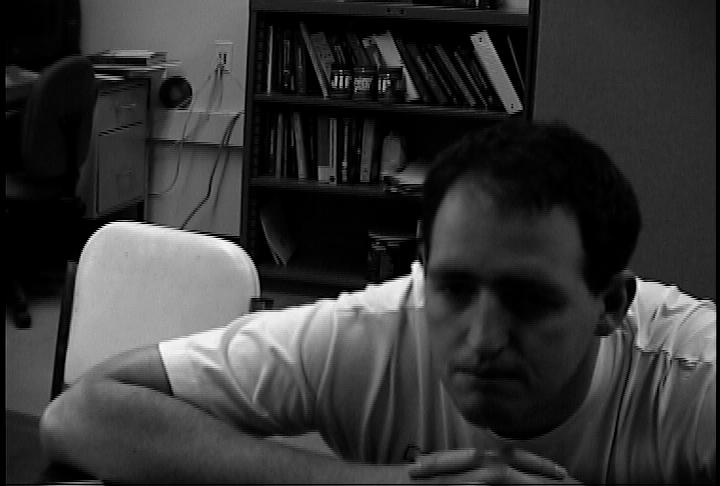
\includegraphics [width=4in]{revRecover.jpg}
\end{center}
\caption{Recovered Image.  This image is the recovered image.  Depending on whether the image was saved as a picture first can affect the white spots in the picture.  Ringing is also an issue.  }
\label{rightDanRecovered}
\end{figure}

\begin{figure}[htb]
\begin{center}
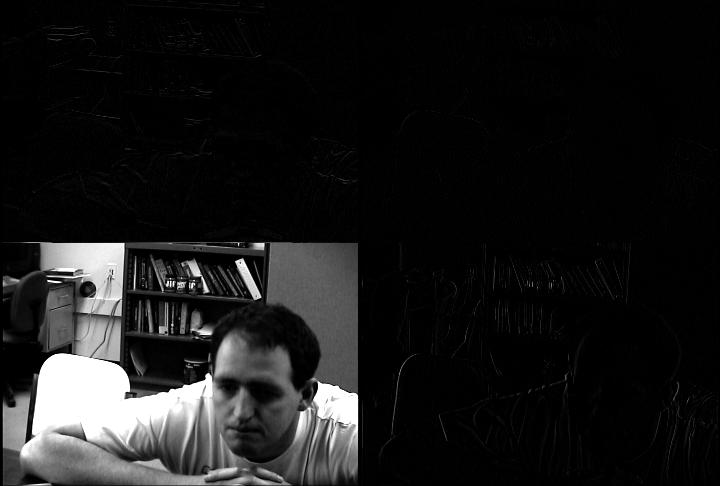
\includegraphics [width=4in]{revWavepic.jpg}
\end{center}
\caption{Wavelet Transform Image.  This image is divided in to average, horizontal, vertical and diagonal components. }
\label{rightWavepic}
\end{figure}

%Note: April 11, 2003:  Proofed up to this point

\begin{figure}[htb]
\begin{center}
\includegraphics [width=4in]{selfWavepic.jpg}
\end{center}
\caption{Wavelet Transform Image.  This image is divided in to average, horizontal, vertical and diagonal components, using the vector-matrix version. }
\label{wavepic}
\end{figure}

\begin{figure}[htb]
\begin{center}
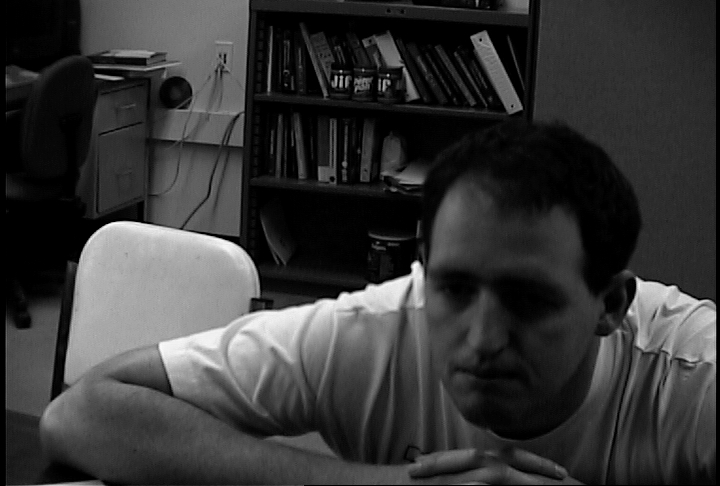
\includegraphics [width=4in]{selfRecover.jpg}
\end{center}
\caption{Recovered Image (Vector-Matrix Method).  This image is the recovered image.  This version avoids the ringing by using the vector-matrix version which is more aligned for the inverse wavelet transform.  }
\label{selfRecover}
\end{figure}

\subsection {Multiresolution}
The expected result is a picture within a picture.  Each average component has a further transform on it.  The three resolution transform has the form:
\[
W_3 = 
\left(
\begin{array}{cc}
\left(
\begin{array}{cc}
\left(
\begin{array}{cc}
A_3& V_3 \\ 
H_3 & D_3
\end{array} 
\right)
V_2 \\ 
H_2 & D_2
\end{array}
\right)
 & V_1 \\ 
H_1 & D_1
\end{array}
\right)
\]
Refer to Figure \ref{wavepicR3} for the image transform results.  

\begin{figure}[htb]
\begin{center}
\includegraphics [width=4in]{wavepic3R.jpg}
\end{center}
\caption{Wavelet Transform Image.  This image is divided in to average, horizontal, vertical and diagonal components using multiresolution wavelet transform.  Note the the average component was transformed one step further. }
\label{wavepicR3}
\end{figure}

\begin{figure}[htb]
\begin{center}
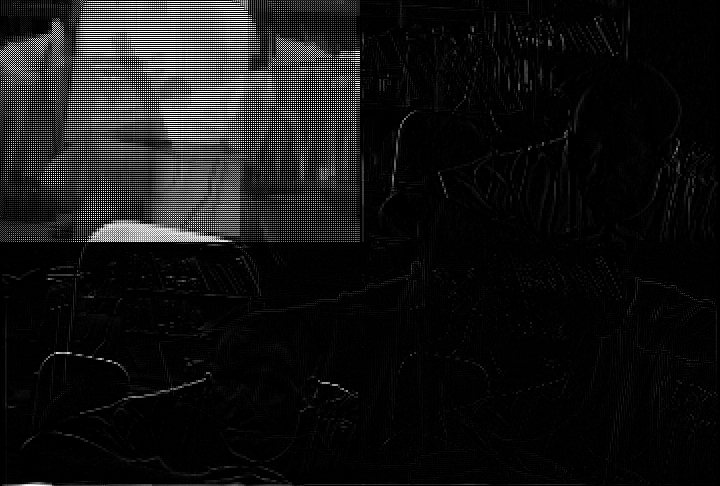
\includegraphics [width=4in]{recoverHid.jpg}
\end{center}
\caption{Recovered Image - Wrong Order (Multiresolution). This image shows a 2D wavelet transform after it was recovered out of order.  Obviously, the distortion is hideous.  }
\label{recoverHid}
\end{figure}

To obtain the inverse, an exact reverse procedure is necessary, otherwise the distortion is hideous.   The first attempt of the wavelet inverse transform was out of order, refer to Figure \ref{recoverHid} .  A correct picture was obtained during the second attempt.  Correct order yielded correct results, refer to Figure \ref{rightDanRecovered}.

\subsection {Threshold Filtering}
After a triple resolution, a 0.02 threshold will eliminate 81.1706 percent of elements in the original sample picture.  Also at this point, the effects of removing these elements becomes visually evident (Figure \ref{recover3R002}).  At a 0.01 threshold,  66.0205 percent of the elements are removed.  Visually, the recovered sample and the original appear to be the same (Figure \ref{recover3R001}).  At a threshold of 0.1, 92.9987 percent of the elements are reduced to zero.  However, the distortions are clearly visible at this level of thresholding (Figure \ref{recover3R010}).  Even at a threshold of 0.001 which is below the numerical precision of the original, 16.0814 elements are reduced to zero.  At a threshold of 0.002, 28.9683 percent is removed.  

Consequently after a triple resolution, nearly 29\% of the data was irrelevant for the image's brightness resolution (which also applies to color).  Subjective examination reveals that removing 60\% to 85\% of the data was not noticeable to human perception.  Which leaves only 15\% to 40\% of the data actually contributing or being necessary to reconstruct the image.   

\begin{figure}[htb]
\begin{center}
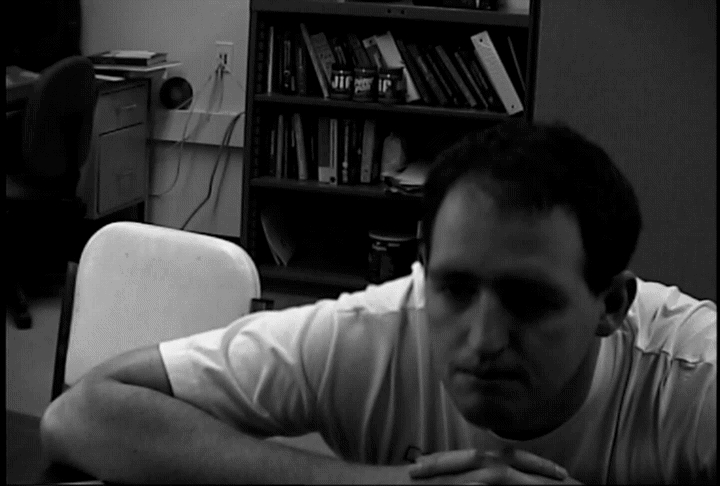
\includegraphics [width=4in]{recover3R002T.jpg}
\end{center}
\caption{Recovered Image - 2\% threshold (Multiresolution). This image had nearly 83\% of its elements removed in the triple resolution wavelet transform.  }
\label{recover3R002}
\end{figure}


\begin{figure}[htb]
\begin{center}
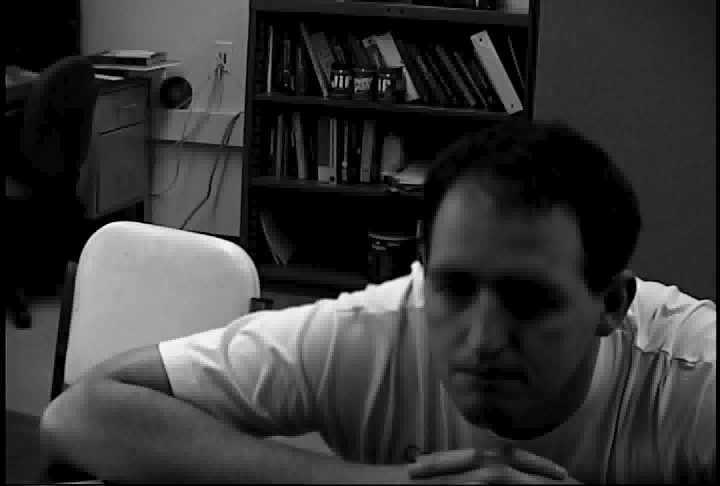
\includegraphics [width=4in]{recover3R010T.jpg}
\end{center}
\caption{Recovered Image - 10\% threshold (Multiresolution). This image had nearly 93\% of its elements removed in the triple resolution wavelet transform.  }
\label{recover3R010}
\end{figure}


\begin{figure}[htb]
\begin{center}
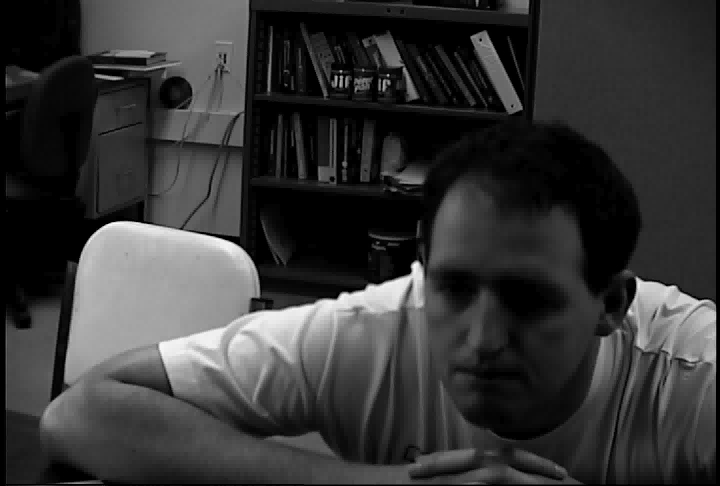
\includegraphics [width=4in]{recover3R005T.jpg}
\end{center}
\caption{Recovered Image - 5\% threshold (Multiresolution). This image had nearly 85\% of its elements removed in the triple resolution wavelet transform.    }
\label{recover3R005}
\end{figure}


\begin{figure}[htb]
\begin{center}
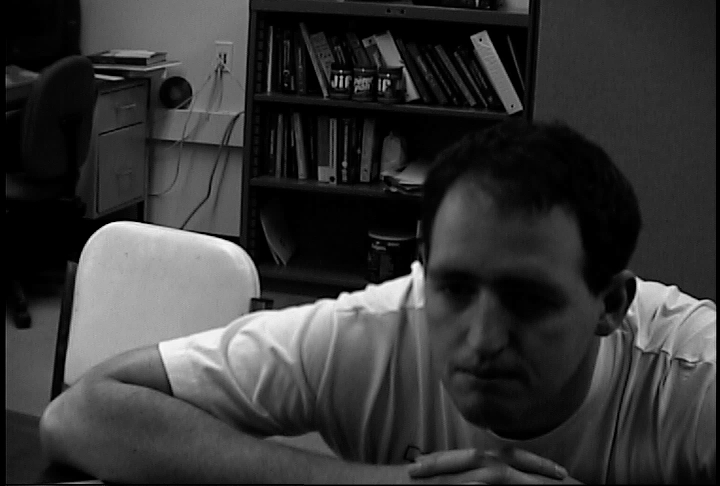
\includegraphics [width=4in]{recover3R001.jpg}
\end{center}
\caption{Recovered Image - 1\% threshold (Multiresolution).  This image had nearly 60\% of its elements removed in the triple resolution wavelet transform.   }
\label{recover3R001}
\end{figure}



%\begin{thebibliography}{99}
%\bibitem{matrix01}Howard L. Resnikoff. and Raymond O. Wells, Jr. \textsl {Wavelet Analysis: The Scalable Structure of Information}  copyright Springer-Verlag New York, Inc.  New York, NY 10010, USA, 1998
%\bibitem{walker}James Walker \textsl {A Primer on Wavelets and Their Scientific Applications}
%copyright Chapman \& Hall/CRC : Boca Raton, FL, USA, 1999
%\bibitem{tabor}Gavin Tabor \textsl {Wavelets - The Idiots Guide} http://monet.me.ic.ac.uk/people/gavin/java/waveletDemos.html
%\bibitem {graps} Amara Graps \textsl {Introduction to Wavelets} http://www.amara.com/current/wavelet.html 

%\end{thebibliography}


\chapter {Matrix Multiplication via Wavelets}
% Note on procedure
%  1.  Make multiplication example W(A) * W(B) = W(A*B) = W(C)
%  2.  Show sparse mechanism for multiplication of two sparse matrices
%  3.  Show design of wavelet based matrix multiplication.  

\documentclass[11pt]{article}
\usepackage{graphicx}
\usepackage{amssymb}
\usepackage{epstopdf}
\DeclareGraphicsRule{.tif}{png}{.png}{`convert #1 `basename #1 .tif`.png}

\textwidth = 6.5 in
\textheight = 9 in
\oddsidemargin = 0.0 in
\evensidemargin = 0.0 in
\topmargin = 0.0 in
\headheight = 0.0 in
\headsep = 0.0 in
\parskip = 0.2in
\parindent = 0.0in

\newtheorem{theorem}{Theorem}
\newtheorem{corollary}[theorem]{Corollary}
\newtheorem{definition}{Definition}

\title{Wavelet Multiplication}
\author{Daniel Beatty}
\begin{document}
\maketitle

\section {Wavelet Matrix Multiplication}

One of the key points for wavelet matrix multiplication is the proof that $W(A) \times W(B) = W(A\times B)$  If this is the case, then it is obvious that $W(A) \times W(B) = W(C) = W(A\times B = C)$.  So far the proof is still weak.  The reason is that an example proof is useful for proving something to not be the case, rather than being the case.   However, a simple example does show some intuitive steps that would be necessary for a proof.  

\subsection{A $2\times 2$ example}
\subsubsection{Conventional Multiplication}

Conventional multiplication is spelled out as

$c_{i,j} = \sum\limits_k a_{i,k} b_{k,j}$

For a $2 \times 2$ matrix, there is the following:
\[
\left(
\begin{array}{ccc}
  a_{1,1}&  a_{1,2} &   \\
 a_{2,1} &  a_{2,2} &   
\end{array}
\right)
\left(
\begin{array}{ccc}
  b_{1,1}&  b_{1,2} &   \\
 b_{2,1} &  b_{2,2} &   
\end{array}
\right) =
\left(
\begin{array}{ccc}
  a_{1,1} b_{1,1} + a_{1,2} b_{2,1}&  a_{1,1}b_{1,2} + a_{1,2}  b_{2,2} &   \\
 a_{2,1} b_{1,1} + a_{2,2} b_{2,1} &  a_{2,1} b_{1,2} + a_{2,2} b_{2,2} &   
\end{array}
\right)
\]

\subsubsection{Wavelet Transform of two $2\times$ 2 matrices}

For a wavelet transform on both matrix A and B, the results are:

\[
W(A) = \frac{1}{2} \left(
\begin{array}{ccc}
  a_{1,1} + a_{2,1} + a_{1,2} + a_{2,2} &  a_{1,1} + a_{2,1} - a_{1,2} - a_{2,2} &   \\
 a_{1,1} - a_{2,1} + a_{1,2} - a_{2,2} &  a_{1,1} - a_{2,1} - a_{1,2} + a_{2,2} &   
\end{array}
\right)
\]

\[
W(B) = \frac{1}{2} \left(
\begin{array}{ccc}
  b_{1,1} + b_{2,1} + b_{1,2} + b_{2,2} &  b_{1,1} + b_{2,1} - b_{1,2} - b_{2,2} &   \\
 b_{1,1} - b_{2,1} + b_{1,2} - b_{2,2} &  b_{1,1} - b_{2,1} - b_{1,2} + b_{2,2} &   
\end{array}
\right)
\]

\subsubsection{Product of A and B in wavelet space}
The conventional product of A and B can be transformed into wavelet space.  The results of this matrix transform is as follows:

\[
W(A\times B) = W
\left(
\begin{array}{ccc}
  a_{1,1} b_{1,1} + a_{1,2} b_{2,1}&  a_{1,1}b_{1,2} + a_{1,2}  b_{2,2} &   \\
 a_{2,1} b_{1,1} + a_{2,2} b_{2,1} &  a_{2,1} b_{1,2} + a_{2,2} b_{2,2} &   
\end{array}
\right) = \frac{1}{2}
\left(
\begin{array}{ccc}
  (a_{1,1} b_{1,1} + a_{1,2} b_{2,1} + a_{1,1}b_{1,2} + a_{1,2}  b_{2,2}) + (a_{2,1} b_{1,1} + a_{2,2} b_{2,1} + a_{2,1} b_{1,2} + a_{2,2} b_{2,2}) &
  (a_{1,1} b_{1,1} + a_{1,2} b_{2,1}  - a_{1,1}b_{1,2} - a_{1,2}  b_{2,2}) +  (a_{2,1} b_{1,1} + a_{2,2} b_{2,1} - a_{2,1} b_{1,2} - a_{2,2} b_{2,2} ) &   \\
 (a_{1,1} b_{1,1} + a_{1,2} b_{2,1} + a_{1,1}b_{1,2} + a_{1,2}  b_{2,2}) - (a_{2,1} b_{1,1} + a_{2,2} b_{2,1} + a_{2,1} b_{1,2} + a_{2,2} b_{2,2})&
 (a_{1,1} b_{1,1} + a_{1,2} b_{2,1}  - a_{1,1}b_{1,2} - a_{1,2}  b_{2,2}) - (a_{2,1} b_{1,1} + a_{2,2} b_{2,1} - a_{2,1} b_{1,2} - a_{2,2} b_{2,2} ) &   
\end{array}
\right) 
 \]
 
 \[ W(A \times B) = 
 = \frac{1}{2}
\left(
\begin{array}{ccc}
  (a_{1,1} b_{1,1} + a_{1,2} b_{2,1} + a_{1,1}b_{1,2} + a_{1,2}  b_{2,2} + a_{2,1} b_{1,1} + a_{2,2} b_{2,1} + a_{2,1} b_{1,2} + a_{2,2} b_{2,2}) &
  (a_{1,1} b_{1,1} + a_{1,2} b_{2,1}  - a_{1,1}b_{1,2} - a_{1,2}  b_{2,2} +  a_{2,1} b_{1,1} + a_{2,2} b_{2,1} - a_{2,1} b_{1,2} - a_{2,2} b_{2,2} ) &   \\
 (a_{1,1} b_{1,1} + a_{1,2} b_{2,1} + a_{1,1}b_{1,2} + a_{1,2}  b_{2,2} - a_{2,1} b_{1,1} - a_{2,2} b_{2,1} - a_{2,1} b_{1,2} - a_{2,2} b_{2,2})&
 (a_{1,1} b_{1,1} + a_{1,2} b_{2,1}  - a_{1,1}b_{1,2} - a_{1,2}  b_{2,2} -a_{2,1} b_{1,1} - a_{2,2} b_{2,1} + a_{2,1} b_{1,2} + a_{2,2} b_{2,2} ) &   
\end{array}
\right) 
\]

\subsubsection{What is $W(A) \times W(B)$}

Straight forward multiplication of $W(A) \times W(B)$ works out as follows:

\[
W(A) \times W(B) = 
\frac{1}{2} \left(
\begin{array}{ccc}
  a_{1,1} + a_{2,1} + a_{1,2} + a_{2,2} &  a_{1,1} + a_{2,1} - a_{1,2} - a_{2,2} &   \\
 a_{1,1} - a_{2,1} + a_{1,2} - a_{2,2} &  a_{1,1} - a_{2,1} - a_{1,2} + a_{2,2} &   
\end{array}
\right)
\times
\frac{1}{2} \left(
\begin{array}{ccc}
  b_{1,1} + b_{2,1} + b_{1,2} + b_{2,2} &  b_{1,1} + b_{2,1} - b_{1,2} - b_{2,2} &   \\
 b_{1,1} - b_{2,1} + b_{1,2} - b_{2,2} &  b_{1,1} - b_{2,1} - b_{1,2} + b_{2,2} &   
\end{array}
\right) = 
\frac{1}{4} \left(
\begin{array}{ccc}
  (a_{1,1} + a_{2,1} + a_{1,2} + a_{2,2})( b_{1,1} + b_{2,1} + b_{1,2} + b_{2,2}) + ( a_{1,1} + a_{2,1} - a_{1,2} - a_{2,2})(b_{1,1} - b_{2,1} + b_{1,2} - b_{2,2}) & 

( a_{1,1} + a_{2,1} + a_{1,2} + a_{2,2}) ( b_{1,1} + b_{2,1} - b_{1,2} - b_{2,2}) + (a_{1,1} + a_{2,1} - a_{1,2} - a_{2,2}) ( b_{1,1} - b_{2,1} - b_{1,2} + b_{2,2})&   \\
 
 ( a_{1,1} - a_{2,1} + a_{1,2} - a_{2,2})(b_{1,1} + b_{2,1} + b_{1,2} + b_{2,2}) +  ( a_{1,1} - a_{2,1} - a_{1,2} + a_{2,2} ) (b_{1,1} - b_{2,1} + b_{1,2} - b_{2,2}) & 
 
( a_{1,1} - a_{2,1} + a_{1,2} - a_{2,2}) (b_{1,1} + b_{2,1} - b_{1,2} - b_{2,2})+( a_{1,1} - a_{2,1} - a_{1,2} + a_{2,2} )(b_{1,1} - b_{2,1} - b_{1,2} + b_{2,2})&   
\end{array}
\right)
\]

Of course this is better simplified.  

\[ \frac{1}{2}
\left(
\begin{array}{ccc}
 (a_{1,1} b_{1,1} + a_{2,1} b_{1,1} + a_{1,2} b_{2,1} + a_{2,2} b_{2,1} +a_{1,1} b_{1,2}  a_{2,1} b_{1,2} + a_{1,2} b_{2,2} + a_{2,2} b_{2,2} ) &
(a_{1,1} b_{1,1} + a_{2,1} b_{1,1} +a_{1,2}b_{2,1} + a_{2,2} b_{2,1} -a_{1,1}b_{1,2} - a_{2,1 } b_{1,2} - a_{1,2} b_{2,2} - a_{2,2} b_{2,2}  )   &   \\
(a_{1,1} b_{1,1} - a_{2,1} b_{1,1} + a_{1,2} b_{2,1} -a_{2,2} b_{2,1} + a_{1,1} b_{1,2} - a_{2,1} b_{1,2} + a_{1,2} b_{2,2} - a_{2,2} b_{2,2} )  & 
 (a_{1,1} b_{1,1} - a_{2,1} b_{1,1} + a_{1,2} b_{2,1} - a_{2,2} b_{2,1} - a_{1,1} b_{1,2} + a_{2,1} b_{1,2} - a_{1,2} b_{2,2} + a_{2,2} b_{2,2}) &   
\end{array}
\right)
\]
 
 Compared with $W(C)$ computed the conventional way:
 
 \[
 W(C) = \frac{1}{2}
\left(
\begin{array}{ccc}
  (a_{1,1} b_{1,1} + a_{1,2} b_{2,1} + a_{1,1}b_{1,2} + a_{1,2}  b_{2,2} + a_{2,1} b_{1,1} + a_{2,2} b_{2,1} + a_{2,1} b_{1,2} + a_{2,2} b_{2,2}) &
  (a_{1,1} b_{1,1} + a_{1,2} b_{2,1}  - a_{1,1}b_{1,2} - a_{1,2}  b_{2,2} +  a_{2,1} b_{1,1} + a_{2,2} b_{2,1} - a_{2,1} b_{1,2} - a_{2,2} b_{2,2} ) &   \\
 (a_{1,1} b_{1,1} + a_{1,2} b_{2,1} + a_{1,1}b_{1,2} + a_{1,2}  b_{2,2} - a_{2,1} b_{1,1} - a_{2,2} b_{2,1} - a_{2,1} b_{1,2} - a_{2,2} b_{2,2})&
 (a_{1,1} b_{1,1} + a_{1,2} b_{2,1}  - a_{1,1}b_{1,2} - a_{1,2}  b_{2,2} -a_{2,1} b_{1,1} - a_{2,2} b_{2,1} + a_{2,1} b_{1,2} + a_{2,2} b_{2,2} ) &   
\end{array}
\right) 
 \]

Notice that $W(A) \times W(B) = W(A \times B) $,  in the case of $2 \times 2$ matrices.

\subsection { Proof of Wavelet Matrix Multiplication}
A reminder from Dr. Sinzinger, wavelets and their inverses are linear operators.  As he correctly reminded me any linear operator has the following properties:

\begin{enumerate}
\item $L(AB) = L(A) \dot L(B)$
\item $\psi ^{-1}$ is a linear operator
\item $\psi ^{-1} (\psi (A) \dot \psi (B)) = \psi ^ {-1} (\psi (A)) \dot \psi ^{-1} (\psi(B)) $
\item $\psi ^{-1}(\psi(A)) = A$
\item $\psi ^{-1}(\psi(B)) = B$
\item Therefore:  $AB = \psi^{-1} (\psi(A) \dot \psi(B))$  
\end{enumerate}

Thus this is sufficient proof that wavelet matrix multiplication is sound.  

\section{Chain Multiplication Structure}
Recall the chain structure.  This structure can be referenced from most introductory algorithm books.  The big idea is to be able to locate specific items quickly by some key which reduces the search to a family of keys that close together by a hashing scheme.  In the case of matrix multiplication, no hash key is needed.  The row or column identifier is sufficient for this.  Of course a description of this scheme is in order.  

Each chain is organized as a one-dimensional array.  Each array has an array list, called a link, which contains the actual data, and array list count showing how many items are in each array.  A next and previous value in this case would be superfluous since columns and rows are arranges in lexicographical order.  The array list contains the following items:
\begin{itemize}
\item key
\item item value (row value/ column value)
\item previous key
\item next key 
\end{itemize}

In the case of a column chain, the keys are row identifiers.   In the case of a row chain, the keys are column identifier.  This structure is similar to a matrix and can be represented by a matrix.  The essential thing for the chain is the arrangement of the array lists.  Zero values are not allowed, and thus order and index keys must be maintained.  

What has this to do with sparse matrix multiplication?  The left matrix is transformed into a row chain and the right matrix is transformed into a column chain.  Each value of the result matrix is simply a multiplication of the row vectors in the left matrix by the column vectors in the right matrix.  With the chain structure, it simply row links times the column links.  Only elements with matching keys are allowed to be multiplied together.  The rest are assumed to be zero, and thus no action is taken.  The sum of the multiplies is the result.  The multiplication procedure is as follows:

\begin{enumerate}
\item Chain Multiply
\begin{enumerate}
\item Arguments: left matrix chain (A) and right matrix chain (B)
\item Results: Result matrix
\end{enumerate}
\begin{itemize}
\item $\forall i \in R.row$
\begin{itemize}
\item $\forall j \in R.col$
\begin{itemize}
\item $R_{i,j} = CM( A[i], B[j]) $  
\item ---- Note that CM is the chain multiply procedure.  
\end{itemize}

\end{itemize}

\end{itemize}

\item Chain Multiply Element
\begin{enumerate}
	\item Arguments:  row link (r) and column link (c)
	\item Output:  Double result: total
	\end{enumerate}
	\begin{itemize}
		\item rlimit = r.size;
		\item climit = c.size;
		\item k = l = 0;
		\item jlow = 0;
		\item total = 0.0
		\item BnotExhausted = true
		\item while both ( k < rlimit) and (BnotExhausted)
		\begin{itemize}
			\item $\forall l \in [jlow, climit)$ if ( $A^c_i . getkey(k) \equiv B^c_j getkey(l)$) then lmatch = l
			\item if ( $l \equiv climit$) BnotExhausted = false
			\item otherwise
				\begin{itemize}
					\item temp += $A^c_i[k] * B^c_i[lmatch]$
					\item jlow = lmatch
				\end{itemize}
		\end{itemize}
	\end{itemize}
\end{enumerate}
					
For the Matrix Chain Multiply the complexity is $O(N^2)$.  For the chain multiply, the complexity is $O(M)$ where M is the larger length of the two links.  Thus total complexity is $O(N^2 M)$ since M's largest size is N.  This a general and simple algorithm for sparse matrix multiplication of matrix chains.  Of course the chore of loading the matrix chains is $O(N^2)$ per matrix.  Thus total cost is on the order of $O(3N^2 M)$.  So long as M is significantly less than N ( on the order of a $\frac{1}{3}$), then the wavelet matrix multiplication has a reasonable advantage.  

\section{Practical Implementation}

There are few questions about the practical implementation that must be answered:
\begin{enumerate}
\item Are the matrices square matrices, and same size?
\item If not, are the dimensions suitable for multiplication?
\item If so, what is the maximum resolution for each matrix?  The lesser maximum is the limit for both.
\item Is the wavelet transform performed on each matrix the same?
\end{enumerate}

A yes answer to the first matrix, allows for an relatively easy transform, and matrix multiply.  If the matrices are not square, then practical problems exist.  If the wavelet transform is the same on each, then the linear proof is sound.  However, if they are not then the proof is bogus and the multiplication is too.  

The general wavelet based matrix multiply is as follows:
\begin{enumerate}
\item Arguments:  
\begin{itemize}
\item A :  a $m \times p$ matrix
\item B: a $p \times n$ matrix
\end{itemize}
\item Results:  C : a $m \times n$ matrix
\item Procedure:
\begin{itemize}
\item $ A \stackrel{\psi}{\to} \alpha$
\item $ B \stackrel{\psi}{\to} \beta$
\item $ \alpha \stackrel {Chain Row}{\to} \alpha ^c$
\item $ \beta \stackrel {Chain Column}{\to} \beta ^c$
\item Chain Multiply ($\alpha ^c , \beta ^c$) $\to C$ 
\end{itemize}
\end{enumerate}

\subsection{Chain Row and Chain Column Setup}
Setting up the the chain-link structure for row or column orientation is relatively simple.  Each one requires proper addressing of the hooks.  The procedures are as follows:

Row Chain-Link Setup
\begin{itemize}
\item $\forall i  \in \alpha .rows$
\begin{itemize}
\item $\forall j \in \alpha . columns$
\begin{itemize}
\item if ( $\alpha [i][j] \approx 0 $)
$a^c.hook_i . addlink(j,\alpha_{i,j} ) $
\end{itemize}

\end{itemize}

\end{itemize}

Column Chain Link Setup
\begin{itemize}
\item $\forall i  \in \alpha .rows$
\begin{itemize}
\item $\forall j \in \alpha . columns$
\begin{itemize}
\item if ( $\alpha [i][j] \approx 0 $)
$a^c.hook_i . addlink(j,\alpha_{i,j} ) $
\end{itemize}

\end{itemize}

\end{itemize}

One of the big questions is how to optimize wavelet packets for multiplication applications.  A straight multi-resolution wavelet on a square matrix is seemingly trivial.  In the square matrix, straight multi-resolution case the number of resolutions is dictate by the size of the matrices being multiplied.  For wavelet packets on square matrices, it is also a size issue.  One can apply wavelet packets to maximum extent that the matrix size allows.  However, some of the packet levels may be unnecessary since the amount energy shuffling is small in comparison to the number of operations.  In the case of non-square matrices, best fits must be applied to ensure that the same wavelet transform 

The Chain-Link Structure

The chain link structure is derived from 2 other classes (hooks and links).   Each one of these classes are relatively simple and can be implemented with either arrays or pointers.  Due to the anticipated size, the array mechanism is chosen for speed and efficiency.  

Class Chain Link members
\begin{itemize}
\item length 
\item hooks
\end{itemize}

Class Hook 
members:
\begin{itemize}
\item length
\item l2norm
\item links 
\end{itemize}



Class Link
members: 
\begin{itemize}
\item id
\item value
\end{itemize}


Recursive Wavelet Packets
The algorithm for optimal wavelet packets is easiest to describe by recursive means.  The stop condition either when the maximum resolution has been reached, or energy shuffle metric is satisfied.  

procedure wavepack (matrix A, integer res) return $\mu$
\begin{itemize}
\item if ($res \equiv 0$  ) stop
\item if ( $A.row {modulo} 2 \equiv  0$ and $A.col {modulo} 2 \equiv 0$) stop
\item if ( optimum) stop
\item otherwise 
\begin{itemize}
\item $A \stackrel{\psi}{\to} \mu $
\item $\mu \stackrel{topleft}{\to} \alpha$
\item $\mu \stackrel{lowleft}{\to} \beta$
\item $\mu \stackrel{topright}{\to} \gamma$
\item $\mu \stackrel{lowright}{\to} \delta$
\item wavepack ( $\alpha$ , res -1)
\item wavepack ( $\beta$ , res -1)
\item wavepack ( $\gamma$ , res -1)
\item wavepack ( $\delta$ , res -1)
\item insert ($\alpha  \stackrel{topleft}{\to} \mu$)
\item insert ($\gamma  \stackrel{topright}{\to} \mu$)
\item insert ($\beta  \stackrel{lowleft}{\to} \mu$)
\item insert ($\delta  \stackrel{lowright}{\to} \mu$)
\item stop
\end{itemize}

\end{itemize}

The determining of the optimum condition is matter that is not well defined. 


 \end{document}




%\chapter {Matrix Inversion via Wavelets}
%\input{inverse}

\chapter {PDE via Wavelets}

%In most of the literature, 
Wavelets are used to condition the difference equation matrix and yield a %better conditioning of the 
sparser matrix.  What this conditioning means is that a wavelet enhanced matrix is easier to solve.  How is this enhancement accomplished?  The condition number is an indication of how quickly a solution will converge.    Sparseness refers to the large concentration of zeroes in the matrix.  Consequently, a sparse matrix has fewer elements to be used in a computation.  The point of this chapter is show how wavelets can be applied to yield a well-conditioned and sparse matrix, how conventional methods of solving PDEs work,  and why a wavelet transformed matrix works for the solution.  Also included is a comparison between conventional and wavelet based methods.  

%This is useful %in
%for increasing the likely hood that the matrix can solved.  %Also, for some implicit forms, 
%Sparse matrices, like those generated by the wavelet transform, are less complex and easier to solve in the case of implicit forms.  %Wavelets can make the matrix even more sparse.  
%When this is the case, 
%In these cases, fast algorithms %can be 
%The reason is that sparse and well conditioned matrices allow fast algorithms to be applied.
%are applied.  
%The goal of this chapter of this thesis is to explore these %softening
%sparse matrix producing  and conditioning techniques that wavelets offer in comparison to traditional methods.  

%\section {PDE in General}
\section {Overview of PDE}
What are partial differential equations (PDE) good for?  
Partial Differential Equations are used to describe several types of systems.  
%Computational Scientists consider partial differential equations (pde) important their ability to 
% PDE could use a s to enforce plurality 
PDE are used to solve %problems as they relate 
equilibrium, diffusion states, and oscillitory systems.  Most %of the
conventional algorithms are computationally expensive %costly 
for performing these tasks.  Therefore the challenge is computing %how to compute 
the solution of PDE with greater speed and accuracy.
%faster.
%these faster has computational scientist concerned.  This why the use of wavelets are considered.  


\subsection {Classic Methods}
%In the classic sense computational scientists agree that 
There are three basic %classification
categories of partial differential equations: elliptical, parabolic, and hyperbolic.  Some scientists consider the hyperbolic to %be made of 
contain a fourth category, ultra-hyerpbolic.  %Regardless, 
Similar properties exist for these groups of problems.  Properties include their boundary conditions and the physical phenomena the PDE models.  %These kind of problems are grouped together for the similarities in properties and boundary conditions. % Also, these classes of PDEs have their own methods for solving them, which are subtly different from each other.  
%Also, three of these types have their own usefulness as they model physical phenomena.  

%For example, 
Elliptical PDE represent %have examples in 
heat expansion, electrostatic charge, and other source expansion problems.  Parabolic PDE model diffusion of gases or fluids.  Oscillating states such as electromagnetic fields, some control theory, vibrating strings, and electronic communication systems all map to the model of hyperbolic PDE.%involve hyperbolic PDEs to model their behavior.  

The general form of second order partial differential equations is %difference for second order partial differential equations is defined % from their general form:

\begin {equation}
Au_{xx} + Bu_{xy} +Cu_{yy} +Du_{x} + Eu_{y} + Fu = G
.
\end {equation}


For the case where $B^2 - 4AC > 0 $, %then 
the PDE is hyperbolic, and the solution has an oscillatory nature to it.  In cases where  $B^2 - 4AC < 0 $,  %then 
the PDE is elliptical.  If $B^2-4AC =  0$ %there is an equivalence to zero, then
the PDE is parabolic.  These classifications determine how the PDE is represented and solved in both the analytical and numerical cases.  %The effect this has on classic methods (analytical and numerical) is how the PDE is represented and eventually solved.  


In addition to the above classifications, %the means of 
their limits or boundaries also have a classification.   Boundary conditions are defined either on the dependent variable or the gradient of the dependent variable.  If %it is the case that 
the specified boundary values produce an open region,  %If the boundary conditions leaves the region open, 
then the problem is an initial value problem.   %These classifications are defined on the method of dependent variable definition.  
%The following are those categories:
%\begin{itemize}
%\item Elliptical (Equilibrium States)
%\item Parabolic (Diffusion states) 
%\item Hyperbolic (oscillating or vibrating states)
%\item Ultra-Hyperbolic 
%\end{itemize}


Boundary conditions for %elliptical
PDE%s
 consist of three categories %check spelling: 
 Dirichlet, Neumann, and Robbin's.  Dirichlet Boundary conditions are specified by either functions or constants on the solution function itself.  Neumann Boundary conditions specify against the derivative of the function based on some either independent or dependent variable.  The combination of the two is called Robbin's Boundary Conditions.  %What does mean?

The following are examples of Dirichlet, Neumann and Robbin's method, respectively% order:
\begin{itemize}
\item $u_n =g(t) $
\item $u = g(t) $
\item $u_n + \lambda u = g(t)$
\end{itemize}



%Subtle differences exist in the solutions to these problems and due to nature of  the problems.  
Each solution (analytic or numerical) is tailored to the equation; however, the three main categories will have similar solutions due to similarities in the problem. 
%can be tailored to fit the specific equation.  
In numerical terms there are two general mechanisms for solving these equations: explicit and implicit.  Explicit tends favor initial value problems and has difficulties with round off errors.  Implicit handles error quite well; however, complexity %exists
 increases depending on the number points to be solved for.  A third method also exists, Monte Carlo.  However, the Monte Carlo method is more for simulating the results of differential or integral equations.  




\subsubsection {Elliptical Differential Equations} 
%One example type that shows up for Elliptical PDE problems is heat conduct, gravitational, electric field, and other static problems.  
Elliptical PDEs can be represented with Poisson's formula.  In the homogenous case, Laplace's equation is the representing equation:
%in the homogeneous case.

\begin{equation}
\frac{\partial ^2 T} {\partial x^2} + \frac{\partial ^2 T} {\partial y^2} = 0
\end{equation}


Also, it is typical for a polygon to be chosen to define the boundary conditions.   Typically, the polygon is defined by constants in either the first derivative or normal space.  %An example would be
The simplest case is a rectangle specified in the first derivative for the right and top edges and constants for the lower and left edges.  Also, the central difference formula is used to setup a linear set of equations to be solved.  \cite{appliedmethods}.  The trick is to set up the matrix and then solve it. % by any means (classic or wavelet based).  

%Boundary conditions for %elliptical
%PDEs consist of three catagories: Dirichlet, Neumann, and Robbin's.  Dirichlet Boundary conditions are specified by either functions or constants on the solution function itself.  Neumann Boundary conditions specify against the derivative of the function based on some either independent or dependent variable.  The combination of the two is called Robbin's Boundary Conditions.  What does mean?

Boundary conditions define the starting point and limits for solving PDEs.  This condition is necessary to have enough constants in the solution for a solution to be calculated.  Different boundary condition types have different methods of solution to account for the boundary conditions.  

\subsubsection {Parabolic Differential Equations}
The parabolic type of differential equations usefully describe diffusion and fluid mechanics.  Some analytical methods useful for solving parabolic equations include substitution of variables as well as Laplace and Fourier Transforms.  Examples of parabolic equations include heat diffusion, diffusion - convection, and Navier-Stokes.  

%Boundary conditions for parabolic PDEs are less formal than elliptical PDEs.  Boundary conditions are specified either across the boundary, on the boundary, or a hybrid of the two.    The boundary conditions are typically spelled by example in temperature equations.  However; it is conceivable that other diffusion problems have similar issues.  

\subsubsection {Hyperbolic Differential Equations}
The hyperbolic type of differential equations are prevalent in equations for oscillating phenomena.  This includes electromagnetic fields and vibrating strings.   In its analytic %al 
form, the D'Alembert Solution is an textbook example method.  The D'Alembert Solution is an example of the canonical form and is used in solving PDE problems.  

% Proofed up to this point 16:07 Friday 

In some literature the canonical form is used to generate a sparse domain.  The general rule for using the canonical form comes from the D'Alembert Solution which is as follows:
\begin{enumerate}
\item Replace (x,t) by new canonical coordinates.
\item Solve the transformed equations.
\item Transform the solution into the original coordinates
\item Substitute the general solution into the initial conditions (IC) and %the
 acquire the constants. 
\end{enumerate}

%\subsubsection {PDE Boundary Value Problems}



 

Some of the boundary conditions that Farlow \cite{PDEfSE} refers to are controlled end points, force specified boundaries, and elastic attachments.  For these force specified boundary conditions, %in the case of force specified points,
 the boundary point itself can move in position.  In the elastic attachment problem, the force can change on each of the boundary points.  %While, 
 %Controlled end points are straight forward functions or constants.  % page 147
Controlled end points are constants or functions on the solution.   
In each case, the force, position, and function of the boundary conditions must be accounted for through out the solution of the PDE.   It is unknown yet as to whether this information will be used in solving any problems in the thesis itself.  

\subsection {Solutions to PDE}

\subsubsection {Difference Equation Formulae}
There are a few formulae used to convert PDE in to their difference equation form.    These formulae are a necessary first step to make a differential equation computable.  The type of of difference formulae is determined by the type of problem.   Each of these come from limits taken to include an $h$ value that moves the index.  If the formula is based on an $+h$ then the forward difference formula is the natural result.  Likewise, $-h$ is the natural result for the backward difference formula.  Central difference is a hybrid of both.  For Central Difference there is a formula for the second derivative as well.  

Central Difference Formula:
\begin{enumerate}
\item \[f'(x) \approx \frac{f(x+h) - f(x-h)}{2h} \]
\item \[f''(x) \approx \frac {f(x+h) -2f(x)+ f(x-h)}{h^2}\]
\end{enumerate}

Backward Difference Formula: 

\[f'(x) \approx \frac{f(x) - f(x-h)}{h} \]

Forward Difference Formula
%\begin{itemize}
%\item 
\[f'(x) \approx \frac{f(x+h) - f(x)}{h} \]
%\end{itemize}


\subsubsection {Explicit Methods/ Iterative Methods}
Explicit methods compute the solution of PDE by using the previous result to compute the current result.  The first step is to  %is 
%to 
acquire %the solution %is%
the transform of the PDE %to
in  its difference equation equivalent.   Any of the difference equations can be used to acquire this form.  %What is important?  
The one line system of eqaution and initial value formula are critical for setting up the remaining solutions. %are used to calculate one result after the next of partial differential equations.  One thing that both implicit and explicit methods have in common is to transform the PDE in difference equations.  At the heart of both methods is the central, backward, and forward difference approximation formulae.  The central difference method is applied to part of a grid with accuracy of $O(x^2)$ and $O(t^2)$.  To illustrate the explicit method, a parabolic PDE used for reference.  That PDE is as follows: %An example of a parabolic equation is used to illustrate this method.  When substituted into the simplest parabolic form;  the new form is 

%Example Method:
%\begin{itemize}
%\item $\phi _{i,j+1} = \phi _{i,j+1} + \frac{2\alpha^2 \Delta t} {\Delta x^2}  (\phi _{i+1,j} -2 \phi _{i,j} + \phi _{i-1,j})   $
%\item $\phi _{i,j+1} = p \phi _{i+1,j} + q \phi _{i,j} + r \phi {i-1,j} $ such that $p,q,r > 0$ and $ p + q + r \le 1$
%\end{itemize}
%$\phi _{i,j+1} = \phi _{i,j+1} + \frac{2\alpha^2 \Delta t} {\Delta x^2}  (\phi _{i+1,j} -2 \phi _{i,j} + \phi _{i-1,j})   $

%$\phi _{i,j+1} = p \phi _{i+1,j} + q \phi _{i,j} + r \phi {i-1,j} $ such that $p,q,r > 0$ and $ p + q + r \le 1$.  

One method is defined for two independent variables.  The solution is started from the set initialized points.  These points already have values as specified by the problem.  The solution is computed from these values.  Then next set of boundary conditions are calculated relative to the next solution.  This procedure is followed until the field is exhausted.   

If the x and t are independent variables, then the following outline is a more specific example of the explicit method.  
\begin{enumerate}
\item Start with the index value of 0 (i=0 at the initial value)
\item Find the solution for all of x for $t=t_{i+1} $ by explicit formula.
\item Establish the boundary conditions with respect for $u_{t_{i+1} ,x}$ by boundary condition approximation formula.
\item Repeat steps 2 through 4 until i = n (where n is the maximum index).
\end{enumerate}

%Typically the explicit formula is composed of the central difference formula for the PDE being solved.  The boundary condition formula is established as the difference formula of all boundary conditions which are not constants.  

%In this case the 
The explicit method is used to solve a PDE where parts of it have been transformed into its central difference equivalent.  The boundary conditions must also be computed in cases where they are not constants.  In cases where the boundary conditions are specified on a derivative, those conditions must be placed in their difference equation form.  %Note that for each iteration, the boundary condition must be computed.

The strength of the explicit method is its speed.  It is a top-down dynamic algorithm which uses only a few previous results to compute the next result.  Thus each result is computed quickly.  However, the
%This computation is useful for cases where speed is necessary.  This method's speed comes from the next step being computed from the current and previous steps.   However, the %is 
explicit form is unstable, and tends to yield results inconsistent with the boundaries.   In order for this form to be stable a reasonable $\Delta x$ and $\Delta t$ must be chosen.  


%Limits on the explicit Method and alternatives by implicit methods are as follows:  
%\begin{enumerate}
%\item Imposed limits on $\Delta x$ and $\Delta t$.  Dependences in explicit methods are directly limited to 3 values of the many values which it theoretically should.
%\item The implicit method is approximately the second derivative $\frac{ \partial ^2 \theta }{\partial x^2} |_{i,j} $ ``by the finite difference formula involving $\theta$ at an advanced time ($t_{j+1}$)''  \cite {appliedmethods}.  A mid-point is computed using a central - difference formula 

%	$\frac{\partial \theta}{\partial t} | _{i,j+1/2} = \frac {\theta_{i,j+1}  \theta_{i,j} }{\Delta t}$
	
%\item The 2nd p.d. applied with central-difference formula.  There is catch with a weighting parameters.  
%\item Variable Weighted Implicit Formula can be used with the following conditions:
%\begin{itemize}
%\item weighting factor $\theta$
%\item more than one unknown variable at the time step $ j+1$
%\end{itemize}

%\end{enumerate}

% Proofed up to this point Nov 3 10:05

\subsubsection{Implicit Methods}

One area where explicit and implicit methods differ is the arrangement of the linear equations used to solve the system.  %Typically, explicit methods utilize the previous solution to determine the boundary conditions of the current solution.   
While in a sense both use linear equations, implicit methods are computed as a system of equations. %lend themselves to simultaneous solution more than explicit ones.    
The implicit method can be computed for a grid of any size.  This is different from the explicit method where the change in value from one index to the next has to be within a narrow range.  

An example of an implicit method is the Crank-Nicolson Method,  a %The idea is to solve by use of a 
system of equations arrived at by converting the PDE into a system of difference equations.   

The Crank-Nicolson Method is performed by the following steps:
\begin{enumerate}
\item Pick some value for $\lambda$ such that $\lambda \in [0,1] $
\item Pick $\Delta x$ and $\Delta t$ and assign grid points
\item Use computational molecule to generate equation.
\item Solve the matrix
\end{enumerate}



\subsubsection {Galerkin}
There is a special case of the implicit method which attempts to optimize the matrix before solving it.  The Galerkin method supposes that a complete orthonormal system $\{v_j\}_j$ is defined on $L^2([0,1])$ and every $v_j$ is $C^2$ on [0,1].  The boundary conditions of the $v_j$ are defined as well.  %is typically defined as well.  
The solution approximation is then defined on the span of this orthonormal system.  For example,
$u_s = \sum_{k\in \Lambda} (x_k v_k )\in S$ such that S is a span of $v_j : j\in \Lambda$, $\Lambda$ is a subset of the natural numbers and $x_j$ is a scalar.  %The catch
However, the necessary condition is that $u_s$ should behave as true solution a system of linear equations, i.e. a vector itself.   The linear equations are %is 
the implicit set of equations for solving a PDE or ODE.  

Frazier takes this one step further to show a parallel from Galerkin to a conventional implicit form.  If L is a linear operation then %First he shows:
%\begin{itemize}
%\item $\langle L u_s, v_j \rangle = \langle f, v_j \rangle$ $\forall j\in \Lambda$ such that $\langle f, g \rangle = \int ^1 _0 f(t) \bar{g(t)} dt $ 
%\item Furthermore: $\langle L (\sum_{k\in \Lambda} x_k v_k), v_j \rangle = \langle f, v_j \rangle$ $\forall j\in \Lambda$ leading to
%$\sum_{k\in \Lambda} \langle L v_k , v_j \rangle x_k = \langle f, v_j \rangle$ $\forall j\in \Lambda$ 
%\end{itemize}
$\langle L u_s, v_j \rangle = \langle f, v_j \rangle$ $\forall j\in \Lambda$ such that $\langle f, g \rangle = \int ^1 _0 f(t) \bar{g(t)} dt $ .
Furthermore: $\langle L (\sum_{k\in \Lambda} x_k v_k), v_j \rangle = \langle f, v_j \rangle$ $\forall j\in \Lambda$ leading to
$\sum_{k\in \Lambda} \langle L v_k , v_j \rangle x_k = \langle f, v_j \rangle$ $\forall j\in \Lambda$ .

%Consistent method of introducing equations Proofed upto this point November 4, 2003

The final connection is that each element of a matrix A defined as $A=(a_{j,k} )_{j,k \in \Lambda}$ is a scalar defined by  $\langle Lv_k , v_j \rangle$.  This connection yields the following equality:

\[(a_{j,k} )_{j,k \in \Lambda} = \langle Lv_k , v_j \rangle ,  \forall j\in \Lambda\] and \[\sum_{k\in \Lambda} a_{j,k} x_k = y_j,  \forall j\in \Lambda\]

The values of this equation are as follows:
\begin{itemize}
\item x is a vector $(x_k)_{k\in \Lambda}$
\item y is a vector $(y_k)_{k\in \Lambda}$ 
\item $A$ is a matrix with rows and columns indexed by $\Lambda$
\item $a_{j,k}$ is an individual element of $A$

\end{itemize}

With Galerkin, for all subsets in $\Lambda$ we obtain an approximation $u_s \in S \to u$.  Such an approximation is obtained by %This is done 
 solving $Ax=y$ then using x to determine $u_s$.  The primary issue %One of the tricks
 is finding  the $v_j$'s and $x_j$'s such that the equations are satisfied.  

Frazier points %ed
 out that the Galerkin method produces a sparse and well conditioned %number
 matrix. %such that condition numbers range from one to infinity. 
   If a wavelet operator is applied, the idea is that the condition number and sparseness will be at a level such that convergence is assured for a given system.  %This is one of the hypothesis to be tested. 
   
  

\subsection {Application of PDE}
The previous subsection discussed PDE in general and how to solve them.  Listed in this subsection are some common PDE problems.  This section has at least one problem of each of the three PDE categories.  In this section, the classic method of solution is applied.  However, the wavelet methods are saved for the next section.  Implicit and Galerkin solutions are generally chosen where accuracy is required, and explicit methods are shown when speed and complexity are necessary.  

In order to make these solutions a few formulae need to be defined.  These formulae are the central difference, forward difference, and backward difference formulae.   Such definitions were provided in the section Difference Equation Formulae earlier in this section.  


\subsubsection {Semi-Infinite String Problem}
The semi-infinite string problem is a typical resonance problem.  Newton's physical laws derive the equation based on external forces, friction forces, restoration forces, and net forces.   In the simplest form, the problem is solved for net forces only.  %Even this problem requires a matrix to solve it.  
The problem is defined mathematically as:

\begin{itemize}
\item PDE $u_{tt} = c^2 u_{xx}$  $\forall x \in (0, \infty)$ and $\forall t \in (0,\infty)$ 
\item BC $u(0,t) = 0$
\item IC $u(x,0)= f(x)$
\item $u_t (x,0) = g(x)$
\item general solution: $ u(x,t) = \frac{1}{2} [ f(x-ct) + f(x+ct)] + \frac{1}{2c} \int ^{x+ct}{x-ct} g(\zeta) d\zeta$
\item $c^2 u_{xx} $ is the net force due to the tension on the string
\item $u_{tt}$  represents the longitudinal or torsional vibrations on the string
\end{itemize}

There is a conventional solution that comes from the central difference, and forward difference formulae.  The rest is rather simple algebra.  One key issue is the boundary conditions.  Boundary values must %These must 
be solved to establish the constants in the matrix.  Once the boundary conditions %these 
are established, %the solution can be arrived at by conventional methods. 
conventional methods can produce the solution.   The conventional algebra is as follows:

\begin{itemize}
\item $u_{xx} = u[i,j+1] - u[i,j] + u[i,j-1] $
\item $u_{tt} = u[i+1,j] - u[i,j] + u[i-1,j] $
\item $u_t = (u[i+1,j] - u[i,j]) $
\item $u[t,0] = 0 $
\item $u[0,x] = f(x) $
\item $u_t [0,x] = g(x) = u [1, x] - u[0,x] $
\item $u[1,x] = g(x) + f(x) $
\item $ u[i+1,j] + (c^2 - 1)u[i,j] + u[i-1,j] - c^2u[i,j+1]  - c^2 u[i,j-1] = 0 $
\end{itemize}



\subsubsection {Heat Diffusion}
%Examples of two point diffusion problems are heat diffusion problems.   In this problem, time and location are the independent variables, and temperature is the dependent variable.  Such a model depends on two constants, the two diffusion points.  

The heat diffusion or heat conduction equation defines heat in a solid at any point and any time within the domain.  Diffusion comes from a heat source, and may come from an artifical constant.  In the case of heat diffusion, there is a constant $\alpha$ which is defined as the diffusitivity constant.  Diffusitivity is defined by the following:

\[\alpha = \frac{K}{\tau \sigma} \]

such that K is the thermal constant, $\tau$ is the density and $\sigma$ is the specific heat.  The heat diffusion problem is defined as follows:


\begin{itemize}
\item $u_t = \alpha ^2 u_{xx} $ such that
\item $u_t$ is the change in temperature with respect to time
\item $u_{xx}$ is the concavity of the temperature
%\item Difference equations for this starts with $u_{xx} = \frac{1}{\Delta x} [u_{i,j+1} - 2u_{i,j} + u_{i,j-1}] $.  
\end{itemize}

\subsubsection {Diffusion - Convection }
%The big idea for 
Diffusion - convection is a description of how %that %regards 
convection currents affect the diffusion process.  In particular, this concept addresses substances diffusing in areas where currents exist.  One case is a gaseous substance being released in an air conditioned room or wind area.  Another case is the release of a liquid substance into a river.  The general formula for diffusion convection is as follows:


\[ u_t = \alpha ^2 u_{xx} - vu_x \]  
where 
\begin{itemize}
\item %where 
$u_t $ is the change in time
\item $\alpha ^2 u_{xx} $ is the diffusion component
\item $vu_x$ is the convection component
\item v is the velocity of the convection current
\item $\alpha$ is the diffusitivity constant
\end{itemize}

% Proofed November 5, 2003 .  Watch for this type intros

The solution to this problem is best done by considering the general solution, and then filling in the constants with the boundary conditions.  The general solution is as follows:

\begin{itemize}
\item $u_t = \alpha ^2 u_{xx} - vu_x $
\item $u_t  =  u[i+1,j] - u [i,j]$
\item $u_x = u[i,j+1] - u[i,j] $
\item $u_{xx} = u[i,j+1] - 2u[i,j] + u[i,j-1] $
\item $u_t - \alpha ^2 u_{xx} - vu_x = 0$
\item $ u[i+1,j] - u [i,j] -  \alpha ^2 u[i,j+1] + \alpha ^2 2u[i,j] - \alpha ^2 u[i,j-1] - v u[i,j+1] + v u[i,j] =0$
\item $ u[i+1,j]   \alpha ^2 u[i,j+1]  - \alpha ^2 u[i,j-1] - v u[i,j+1] + (2 \alpha ^2 +v - 1)  u[i,j] =0$ 
\end{itemize}

%\subsubsection { Electromagnetic Fields Problems}

%\subsubsection {Electrostatic Expansion Problem}
\section {Related Work}

%\subsection {Gregory Beylkin}
\subsection {Sparsifying the Kernel with Wavelets}
One example of applied mathematician in the field of wavelets is Gregory Beylkin of the University of Colorado.  He has published several papers on the topic, and a few of his have similar work to this paper.  %Some of his quotes deserve some explaination, and other do not.  
This paper highlights a few of his quotes and explains their meaning.  The main point is to use the wavelet transform to diagonalize the matrix for fast sparse methods to work.  

One quote, ``Fast algorithms for applying these operators to functions, solving integral equations.  The operators which can be efficently treated using representations in the wavelet bases include Calderon-Zygmund and pseudo-differential operators.''\cite{bvpbeylkin}  This quote references two mathematical forms introduced in the early half of the 20th century.  Calderon-Zygmund was a difference operator that divided the vector in two each time it operated.  The more generic version, the psuedo-difference operator was introduced shortly thereafter.  Both introduced methods of numerically differentiating equations.  Beylkin used kernel K to illustrate the use of the wavelet transform: 

\[T(f)(x) = \int K(x,y) f(y)dy \]

This kernel allows for the mathematical explanation of how wavelets fit in scheme with %of 
solving PDE's.  The bottom line is best said in Beylkin's own words, ``If our starting point is a differential equation with boundary conditions then the wavelet system of coordinates there is a diagonal preconditioned which allows us to perform algebraic manipulations only with the sparse the sparse matrices. ... The wavelets play an auxiliary role in that they provide a system of coordinates where the condition numbers of the sparse matrices (involved in the computations) under control.  ''

Indeed, in Beylkin's examples the wavelets diagonalize the matrices for which it works on.  Beylkin's multi-resolution scheme is unique in the way it provides the diagonalization process.  %It 
Each resolution is performed successively on each average term.  However, the averaging and differencing is applied to portions in the vertical and horizontal components.  Thus, some of these parts are also forced to zero. % It is unknown as to why other multi-resolution techniques are not applied.  Also unknown is how determine an optimum diagonalization of the matrix by the wavelet transform.  

%Another paper of Beylkin had theme that for a number of operators, the non-standard form of wavelet basis could be used to reduce certain problems to a small system of linear equations.  It was highly mathematicall

Belykin claims in another paper that wavelets support rapid application of dense matrix.  In some cases, Beylkin claims to achieve results %operations
 in $O(N^2)$ operations.  In general, it is clear that wavelets offer the ability to reduce the overall size of the input, and therefore reduce the time necessary to compute the result.  It is important to note that the input is an equivalent form to the original, and the new form is simply more compact.  

On both integral applications, it is known that the algorithms have hidden recursive components that tend to make the algorithm grow exponentially.    In cases described by Farlow \cite{PDEfSE}, integral equations are solved in a similar manner to PDE's by using there numerical equivalence forms.  

Lastly, Beylkin points out that wavelets have several advantages over the Fast Fourier Transform (FFT).  Amongst them is the cost of the transform itself.  The wavelet transform in 1-D space has a cost of nearly $O (N)$. where the FFT is of order $O(N^2)$  Another is translation invariance.  The wavelet transform does not require translation invariance, where as the FFT does.  This gives the wavelet transform some adaptability to numerical applications.  




%\paragraph{Methods of the Paper}
%\subsubsubsection { }
%The paper used the Haar Wavelet Transform, and mechanisms first developed by Stromberg, Meyer, and Ingrid Daubechies.  Operators included in the study are integral, Dirichlet and Neumann boundary value problems for elliptical partial differential equations, and  Legendre series.  The idea like most wavelet schemes is to use the wavelet transform to make the matrix operator very sparse.  Once that is the case, the operation against a vector is $O(N)$ in complexity.      The construction is claimed to be $O(N^2)$ with the exception of structures whose singularities are known a priori.  In the case of the exception, the compression operator is an order O(N) procedure.  

%Mechanisms provided that the article claims to provide for evaluating integral operators.  A standard and non-standard form.  The non-standard scheme claims to extend the standard form leading to an $O(N)$ scheme.  

%The paper is organized with section concepts.  The first concept is the Haar Wavelet Basis.  Second are relevant facts regarding wavelets.  Third is a description of the integral operators for which we obtain an order N algorithm.  Included with the third is a billinear operator and its description.  Fourth is the complexity analysis.  Finally, the numerical applications of wavelets are presented.  

%\subsubsubsection
%\paragraph{Properties of Wavelets}
%One property that the article hits on is the fact the Haar Wavelet does not drop off very fast.  In the case of the paper, the Daubechies Wavelet Basis functions are used.  

%\section {Where do Wavelets Fit In}
%In most of the literature, wavelets are used to soften the difference equation matrix, and yield a better conditioning of the matrix.  This is useful in increasing the likely hood that the matrix can solved.  Also, for some implicit forms, Wavelets can make the matrix even more sparse.  When this is the case, fast algorithms can be applied.  The goal of this chapter of this thesis is to explore these softening  and conditioning techniques that wavelets offer in comparison to traditional methods.  

%\subsection {Softener }
%\subsection {Correction Factors}


\subsection {Turbulance and Navier Stokes}
Jaffard, Meyer, and Ryan showed exploration into the basis functions useful for solving PDE problems, such as Navier-Stokes and other turbulance problems.  Amongst the first attempts for solving Navier-Stokes used the Battle-Federbush and Shannon basis.  One of the keys for this problem was the absense of boundary conditions.  

The idea was to apply the Battle-Fererbush basis with the Gelerkin method to solve Navier Stokes.  This concept was first published by Zenin in 1981.  One of the difficulties is getting the matrix solution to diagonal form.  The Shannon basis does not cause the non-diagonal elements to decay rapidly.  In some cases, neither does Battle-Federbush.  

The main issues for wavelets and PDE solutions in some opinions is to address complicated geometries.  In some cases, %Others see that 
local refinements can enhance or be used in place of multi-grid algorithms% in some cases
.   Again, the key is to make the solution matrix converge to diagonal and sparse system.  

%\subsection {Wim Swelden}
%Wim Swelden has published papers of wavelets in the spherical coordinate system.  A few problems this addresses are PDE's on astronomical phenomina with consideration of the spherical system of coordinates.  One example of this was written by Gallegos, Martinez-Gonzolez, Argueso, Cayon, and Sanz.  The example was to solve non-Gaussian features in astronomical images and spectra.  In that case, the Spherical Mexican Hat basis was the best basis function for extracting the information.  

\subsection {KL Transform Approach}
%In the solution of the PDE in implicit form, the bottom line is to solve a linear equation.
All implicit methods place their information into a matrix and then solve that matrix as a system of linear equations.  One approach is to use the Karhunen-Loeve (KL) transform.   As stated by Wickerhauser \cite{victor} the overall goal of this solution method is to acquire the singular values, eigenvalues, and eigenvectors.  From these answers, the solution to the matrix is trivial.  Methods for accomplishing this extraction are factor analysis, principle component analysis, singular value decomposition, and the KL transform.  


%Proofed up to this point at November 6, 2003

The point of wavelets with the KL-Transform was well stated: ``The approximate factor analysis algorithm is the search through a library of orthonormal basis for the one whose H is closest to that of the Karhunen-Lo$\grave{e}$ve basis, and cases of fast search methods the result is a fast approximate Karhunen-Lo$\grave{e}$ve algorithm.  "\cite{victor}  

So what problem is solved by the KL transform?   ``Two problems solved by  principle orthogonal decomposition.  First, distinguishing elements from a collection by making d measurements.  Second, inverting a complicated map from a p-parameter configuration space to d-dimensional measurement space. '' \cite{victor}  What does this mean?  Usual cases for the extraction of singular values depend on the measurements taken.  The parameters necessary to get these values by certain formulae are extracted by their singular values that the KL transform can acquire.  In the case of PDE, these parameters represent a mapping to eigenvalues, eigenvectors, and singular values.  As stated, ``the Karhunen-Lo$\grave{e}$ve basis eigenvectors are also called principle orthogonal components or principal factors, and computing them for a given ensemble X is also called factor analysis.''\cite{victor}

Where do wavelets come in?   ``It is possible to build a library of more than $2^d$ fast transforms U of $R^d$ to use for ``x" points.''\cite{victor}
%Question:  What does this mean?  
 This  built library means that wavelets can be used to construct the fast transforms family designated U which are specific for the point ``x.''  From these bases, a particular wavelet basis can be selected as the best choice. %,  or so this idea is implying.

%Look for plural of basis

The method of using wavelets to acquire the KL transform is stated as follows:  
 \begin{itemize}
\item Expand N vectors $\{X_n \in R^d : n = 1,2, \ldots ,N\}$ into wavelet packets' coefficients: $O(Nd\log d)$
 \item Summing squares into the variance tree: $O(d \log d)$
 \item Searching the variance tree for the best basis: $O(d+d\log d)$, if it exists
 \item Sorting the best basis vectors into decreasing order $O(d \log d)$
 \item Diagonalizing the auto-covariance matrix of the top $d^\prime$ best basis vectors $O({d^\prime}^3)$
\end{itemize}

The total complexity of the Approximate Karhunen-Lo$\grave{e}$ve bases: $O(Nd\log d + {d^\prime}^3)$.  Since $d^\prime \ll d$, it is safe to say the approximate solution is faster than the conventional one. 

The approximate Karhunen-Lo$\grave{e}$ve transform of one vector 
\begin{itemize}
\item Computing the wavelet packet coefficients of one vector $O(d \log d)$
\item Applying the $d^\prime \times d^\prime$ matrix $K^{\prime \ast}$ : $O({d^\prime}^2)$
\end{itemize}

Updating the approximate Karhunen-Lo$\grave{e}$ve basis 
\begin{itemize}
\item Expanding one vector into wavelet packet coefficients 
\item Adding the coefficients into the means tree
\item Adding the squared coefficients into the squares tree
\item Forming the variance tree and computing the new information costs
\item Searching the variance tree for the joint best basis
\end{itemize}

The classification in large data sets applies to both the rogues' gallery problem, fingerprint classification problems, and rank reduction for complex classifiers.  

%\subsection {Galerkin Approach}

%\subsection{The Recursive Multi-Resolution Approach}
\section {Proposed Work}
This chapter proposes to utilize the wavelet transform to pre-condition PDE.  Once a PDE matrix is preconditioned,  the similar matrix is to be solved.  A few wavelet basis functions and multi-resolution methods shall be studied for their properties in preconditioning a matrix.  

The PDE problems to be used are the semi-infinite string, heat-diffusion, and diffusion convection.    In all three cases, the implicit method enhanced with the wavelet transform shall be used.  A straight implicit method shall be used for comparison.  

\subsection {Basis Function Preconditioning Functions}
The primary basis functions to be used as test basis functions are the Haar Wavelet, Daub4, and the Mexican Hat.  The Haar basis function is orthonormal and preserves the data; however, Haar does not cause as rapid convergence as Daub4 or the Mexican Hat.  The Daub4 is bi-orthonormal and has a courser difference term.  %The Mexican Hat is under consideration due to its use in astrophysics on non-gaussian features. 

\subsection {Multi-Resolution Conditioning Methods}
There are two general forms that could be called the Recursive Multi-Resolution Wavelet Transform.  Both of these obey the rule from linear algebra that states that the solution to a matrix A is the same as that of matrix B if B is similar to A.   Where these two forms differ is in their coverage of the matrix.  It is presumed that these two forms can probably be applied to any orthonormal wavelet basis and probably to any bi-orthonormal wavelet basis as well.  

\subsubsection {Procession of Averages}
One form could be called the procession of averages.  It is a form that has been cited in this paper repeatedly.   Each resolution transforms the average term with another wavelet transform until the size of the final average term is too small on which to perform another transform.  %This works for 
The procession of averages works when most of the energy is contained in the average term.

\subsubsection {Recursive Multi-Resolution Quad-Tree Method}
An alternative form recursively works on all four terms.  A quad tree is used to model the recursive process, hence the name the Recursive Multi-Resolution Quad Tree.   In the case of the quad-tree, the stopping point is defined for either when a leaf's energy goes to zero or a leaf's matrix is too small to be transformed.  

An optimal condition is used as the stopping condition of the wavelet transform using the Recursive Multi-Resolution Quad-Tree Method.   %To achieve the primary objectives, an optimal condition has to be defined for the matrix and its quad-tree.  
This condition is used to zeroize the leaves of the quad tree as much as possible.  %The second is the concentrate the energy at the diagonal of the matrix.  %Last is just a hypothesis of using half-transforms.  
Another optimal condition that is desirable is for the energy of the matrix to be concentrated in the diagonal of the matrix.  However, this condition is not guaranteed by any multi-resolution method.   Of course, a matrix in any of the leaves which is not of size to be preconditioned is also a stopping condition.  

%The process of the wavelet transform should separate the high-energy components from the low/zero energy components.  Zero leaves are leaves where the energy of the leaf is below the zero energy threshold.  If this occurs the leaf can be labeled a zero leaf, and this is a terminating condition.  Obviously, non-zero leaves are significant and must be retained.  

%There is one possibility which corresponds to Gregory Belkin's method which is to apply half-wavelet transforms in certain regions of the matrix.  One section to be concerned about is the diagonal component.  In the case of the diagonal and average components, a full-wavelet transform may be necessary to cause the diagonal in those sections to diminish faster. 

\subsection {Evaluation Methodology}
The most obvious issue needed from any of %other
 these conditioning methods is for the end results to be correct.  The answers must numerically match the results obtained by the conventional implicit method.  To test this correctness, each solution conditioned by wavelets are checked against their implicit method counter-part.  

The second issue to test is efficiency.  There already exists the theoretical measure of efficiency.  However, an empirical study is also a result that is of interest.  The number of operations and the memory space consumed shall be considered measures of efficiency.  


%It is true that there are two forms that can be defined as the Recursive Multi-Resolution Wavelet Transform.  This is not referring to the different wavelet basis functions that can be used.  Rather, it is reference to how the multiple resolutions are applied to the matrix to obtain a similar matrix.   Recall from linear algebra that the solution to a matrix A is the same as a matrix B which is similar to A.  



%One form uses a quad-tree to ensure that recursion is applied through-out the matrix.  The other only applies it to the average term recursively.   The obvious difference here is that the second only considerer one branch of the tree to continue recursion on.  The first considers all branches.  The second offers the ability to arrive at a sparse matrix, and determine an optimal matrix.  

%Major Point: Use multi-resolution to eliminate the non-diagonal elements.  In a quad-tree multi-resolution wavelet transformed matrix, many diagonals are expected.  However the majority of the strength is expected to be in the main diagonal.  

%The primary objective of using these forms to solve PDE are to ensure that matrix is transformed into a similar matrix which is well conditioned and is sparse.  %issue that all related research regarding wavelets and partial differential equations is the need to produce a sparse and well-conditioned matrix for solving PDE via the implicit method.  
%In case of a quad-tree, all resolutions and components are available for consideration.  If it is the case that many diagonals are formed then this case must be examined.   One consequence of the primary goal is for a majority of the matrix strength is expected to be in the diagonal.   %Many diagonals are expected, and the majority of the matrix's strength is expected in the diagonal.  Also. many sections are expected to be zero.  


%Zero branches are expected to appear in the first three to seven levels (resolutions).  When this occurs, the result of the computation of the children can be assumed to be zero also.    

% Optimal Conditions: Zeroized Leaves, Concentration on the diagonal, and half transforms



%Concentration of non-zero leaves near the diagonal is the next step in optimization.  Careful measurement of energy of non-zero leaves in non-diagonal sections can be a problem.  One method for consideration is the arrangement of wavelet transform terms to ensure a diagonal matrix.  

%One feature of the 2-D wavelet transform, arrangement of the average, vertical, horizontal, and diagonal terms is relative, but not absolute.  Selection of the average term's corner is arbitrary.  The diagonal is always catty-corner to the average term.  The vertical and horizontal term positions are determined relative to the average term.  

%Zero branches are expected to appear in the first three to seven levels (resolution).  One optimal condition is highest level tree where a majority of the energy of the tree is concentrated in just a few leaves.   The other optimal condition is such that energy of the matrix is concentrated in the diagonal of the matrix.  

%The two optimal cases imply a cross reference condition such that both optimal conditions are satisfied.  In the quad-tree multi-resolution method, this is accomplished by using the tree to reference the boundaries of each individual component, while representing the data in the matrix.    A special value in the quad-tree's data structure should be energy.  When the leaves which correspond the diagonal region have the largest energy, and the sections away from that diagonal have energy sparsely concentrated in just a few leaves, then the matrix is optimized.  

%Possibility of half resolution?

%There is one possibility which corresponds to Gregory Belkin's method which is to apply half-wavelet transforms in certain regions of the matrix.  One section to be concerned about is the diagonal component.  In the case of the diagonal and average components, a full-wavelet transform may be necessary to cause the diagonal in those sections to diminish faster. 

%Application of recursive method in implicit solution.



%********************************************************************************

%\begin{thebibliography}{99}
%\bibitem {appliedmethods} Singiresu S. Rao \textsl{Applied Numerical Methods for Engineers and Scientists}  published Prentice Hall Upper Saddle River, NJ 07458 copyright  2002
%\bibitem {numrecipies} William H. Press, Saul A. Teukolsky, William T. Vetterling, and Brian P. Flannery 
%\textsl {Numerical Methods in C}
%Published by the Press Syndicate of the University of Cambridge The Pitt Building, Trumpington Street, Cambridge CB2 1RP
%40 West 20th Street, New York, NY 10011-4211, USA
%Copyright Cambridge University Press 1988, 1992

%\bibitem {bvpbeylkin}  G. Beylkin \textsl{On wavelet-based algorithms for solving differential equations}

%\bibitem {amsbeylkin}  G. Beylkin \textsl{Wavelets and Fast Numerical Algorithms}

%\bibitem {fwtnal} G. Beylkin, R. Coifman, and V. Rokhlin \textsl {Fast Wavelet Transforms and Numerical Algorithms I, Article in Communications on pure and applied mathematics} copyright 1991 Wiley, New York

%\bibitem {mwabeylkin}  G. Beylkin, D. Gines and L. Vozovoi \textsl{Adaptive Solution of Partial Differential Equations in Multiwavelet Bases }

%\bibitem {PDEfSE} Stanly J. Farlow \textsl{Partial Differential Equations for Scientists and Engineers} copywrite 1993 Dover Publications, Inc Mineola, N.Y. 11501

%\bibitem {spiegel} Murray R. Spiegel, \textsl { Theory and Problems of Advanced Mathematics for Engineers and Scientist} copy-write 1996 McGraw-Hill 

%\bibitem {tools} Stephane Jaffard, Yves Meyer, and Robert D. Ryan \textsl {Wavelets: Tools for Science and Technology} copyright 2001 by the Society for Industrial and Applied Mathematics Philadelphia, PA 19104-2688

%\bibitem {victor} Mladen Victor Wickerhauser \textsl {Adapted Wavelet Analysis from Theory to Software} copyright 2001 by the Society for Industrial and Applied Mathematics Philadelphia, PA 19104-2688


%\end {thebibliography}


% \end{document}

\appendix
\chapter{Wavelets Implemented in General}
\section{Haar Wavelet Transform Class:}

\bigskip The Haar Wavelet Transform class has the purpose of taking in a
signal and outputing the signal processed by the Haar Wavelet Transform. \
It is dependent on the convolution function for computation. \ It is also
dependent on the haar function generator to establish a Haar Scaling and
Wavelet vector. \ For practical I/O, a result plotter is also necessary. \ 

\bigskip All of the above can be accommodated within one class. \ One other
class that is necessary is the myVector class. \ This class provides a
simple, yet practical data type for the computation. \ It can be allocated
and deallocated such that its size is appropriate for the task. \ 

It is projected that the two-dimensional version will simply add a matrix
manipulator. \ What such a manipulator extracts rows and columns into
myVector structures such that the computation to procede on each row and
column.. \ 

\subsection{\protect\bigskip One Dimensional Wavelet Transform}

The primary function in the Wavelet transform class is the one dimensional
wavelet transform (hWaveXform). \ More than one form of this function could
possible exist; however, for simplisty only one was produced. \ It takes two
myVector classes (input and output). \ It produces a haar difference and
scaling vector, as well as a $R_{A}$, $R_{D}$, $T$, $F$ and $S$ myVector
classes for use within the function. \ The algorithm is as follows

$S=input$

$l=$ is the size of S (or the input)

$\forall i\in \lbrack 0,l)$

\qquad $R_{A}=S\ast H_{A}$

\qquad $R_{D}=S\ast H_{D}$

\qquad T = join ($R_{A}$,$R_{D}$)

\qquad F = evenSplit (T)

\qquad ForceInsert (F, output)

\qquad end = floor ( $\frac{l}{2^{i+1}}$)

\qquad Extract (output, S, 0, end)

\bigskip

The Extract procedure is to take values from output up to the index end, and
make S a copy of that vector. \ Thus S is called the resolution vector. \ T
is always twice the size of the working S vector. \ F is always half. \ The
resolution vector decreases by half each iteration, and starts at the same
size as the input.

\bigskip

\subsection{Join Procedure}

The join procedure is rather simple. \ Produce a result whose size is the
size of the two sources combined, and whose elements are those of the two
input vectors. \ 

Input:

\qquad myVector left, right

Output:

\qquad myVector Result

Algorithm

\qquad result.deallocate

\qquad $s_{l\,}=size(left)$

\qquad $s_{r}=size(right)$

\qquad $s=s_{l}+s_{r}$

\qquad result.allocate(s)

\qquad $\forall i\in \lbrack 0,s_{l})$

\qquad \qquad result[i]=left[i]

\qquad $\forall i\in \lbrack s_{l},s)$

\qquad \qquad result[i]= right$[i-s_{l}]$

\subsection{Procedure: Even Split}

This procedure is simply a special type for condensing procedure. \ Simply
put, this procedure makes the result half the size of the original input. \
Both the input and result are myVector classes. \ The characteristic of the
elements of the result is:

\qquad result[i] = input[2*i]

\subsubsection{Input:}

\qquad myVector s

\subsubsection{Output:}

\qquad myVector r

\subsubsection{Algorithm}

\qquad l = ceil (s.size/2)

\qquad r.allocate(l)

\qquad $\forall i\in \lbrack 0,l)$

\qquad \qquad $r_{i}=s_{i\ast 2}$

\bigskip

\bigskip

\subsection{Procedure: Force Insert}

\bigskip Purpose: To insert one myVector ,s, into a larger myVector, r. \
The constraint is that r be larger than s. \ As long as this is the case,
then forced insertion can occur. \ Special cases can include start and end
points. \ In which case, the start and end points must be within the
specified range.

\subsubsection{Input:}

\qquad myVector s, r

\subsubsection{Output:}

\qquad myVector r

\subsubsection{Algorithm:}

\qquad $l_{1}=s.size$

\qquad $l_{2}=r.size$

\qquad if ($l_{1}<l_{2}$) and (start < end)

\qquad \qquad $\forall i\in \lbrack start,end]$

\qquad \qquad \qquad $r_{i}=s_{i}$

\bigskip

\subsection{Procedure: Extract}

Purpose: To produce a new or replace a myVector whose length is that of the
section to copied and extracted. \ The point behind this procedure is
provide allow a wavelet transform to be performed on a segment of data, and
keep the procedure the same each resolution. \ 

\bigskip

\subsubsection{Input:}

The inputs for the wavelet Xform extraction procedure are as
follows:

\qquad myVector S,

\qquad integer a \ 

\qquad integer b \ 

These names are arbitray. \ The variables a and b specify the start and end
points respectively. \ Obviously, there is an inequality relationship here.

\qquad $0\leq a\leq b\leq S.size$

\bigskip

\subsubsection{Output:}

The output of the wavelet Xform > extraction procedure is
simply:

\qquad myVector R

The elements of R are a copy of the elements of S from index a to index b.

\bigskip

\subsubsection{Algorithm}

\qquad if ( 0 <a < b < S.size)

\qquad \qquad R.deallocate

\qquad \qquad l = b - a +1

\qquad \qquad R.allocate(l)

\qquad \qquad $\forall i\in \lbrack a,b]$

\qquad \qquad \qquad $R_{i-a}=S_{i}$

\bigskip


\subsection {Procedure: Haar Wavelet Inverse (Left Side)}
Purpose:  These procedures are specific case toward the 2-element Haar Wavelet.  They take in an array of even length and return an array of equal size which is the Inverse Haar Wavelet Transform of the original.  The format of the original is assumed to be ($A|D_{1}|D_{2}|...|D_{n}$).

\subsubsection {Input}
A "MyVector" class which is an array with simple operations associated with it.   The object name is source.  The source is of the form ($A|D_{1}|D_{2}|...|D_{n}$).  

\subsubsection{Output} 
A "MyVector"  class with an object name of result.  

\subsubsection{Algorithm}
There is a difference between the current algorithm and the ideal algorithm which may be the source of error.  This algorithm uses the following symbols to aide in its description:
\begin{itemize}
\item S is the source myVector
\item A is the average term for which $A_i = S_i$ \newline
\item D is the difference term for which $D_i = S_{i+l/2}$ \newline
\item l is the length of S
\end{itemize}

The first version has the following algorithm:

\begin{enumerate}
\item Initialize the result, R.
\item $\forall i \in [0,\frac{l}{2}]$
	$R_{2i} = (A_i + D_i) \sqrt{ \frac{1}{2}}$
\item $\forall i \in [0,\frac{l}{2}]$
	$R_{2i-1} = (A_i + D_i) \sqrt {\frac{1}{2}} $
\end{enumerate}

There is a problem with this method.  Let us start with the even values:   $R_0 = (A_0 + D_0 )\sqrt{1/2}$.   Now the odd, not that $R_{-1}=(A_0 + D_0)\sqrt{1/2}$ which of course does not exist.  Next, $R_1 = (A_1 - D_1)\sqrt{1/2}$ is valid.   Lastly, $R_{l-1}=R_{2*(l/2) - 1} = (A_{l/2} - D_{l/2})\sqrt{1/2}$.  The problem is that $A_{l/2}$ and $D_{l/2}$ do not exist.  Thus, $R_{l-1}$ does not exist, either.  

\bigskip

\section {2-D Wavelet Transform Class}
This class provides three functions. \ The column wavelet provides a
transform solely on the columns. \ The row wavelet likewise, provides a
wavelet transform on each of the rows. \ The 2-D\ wavelet transform is
simple a row wavelet followed by a column wavelet transform. \ 

It should be noted that these wavelet transforms are Haar Wavelet
transforms.. Multiple resolutions functions can be made, but again it is
still the Haar Wavelet at the core. \ Other class clones may be produced to
use other wavelet basis such as Daubachie or Coeflet. \ 

Another support class required for support of the two dimensional wavelet is
the image reader/ writer. \ Such a class of functions provide means of
acquiring data for a matrix to be computed. \ Granted this matrix could have
been populated by other means. \ Generating such a class consumed some time
on this project. \ The reason is that there a few mechanisms for doing this.
\ One is to use raw image types. \ These types are known as by their
extensions: pgm and ppm. \ Another popular mechanism is Image Magick. \ The
reason for Image Magick is that it is available on most UNIX platforms
(Linux, IRIX, Solaris, and Mac OSX). \ Otherwise, schemes such as Apple's
Quicktime would be used. \ The other reason for the use of other software to
acquire the image is that the objective of this class is not produce image
translators for each image type imaginable. \ 

\subsection{\protect\bigskip Method: Column Wavelet Transform}

The column wavelet transform is provides a source matrix, and returns a
result. \ In order to yield this result, each column is extracted into a
vector and that vector is fed into a one-dimensional transform. \ The result
of the one dimensional transform is placed the corresponding row of the
result matrix. \ Mathematically, this algorithm is as follows:

\qquad $\forall j\in col$

\qquad \qquad n = 0

\qquad \qquad $\forall i\in row$ in reverse order

\qquad \qquad \qquad $S_{n++}=$source$_{i,j}$

\qquad \qquad $S$ ${W}{\Rightarrow }R$

\qquad \qquad n = 0

\qquad \qquad $\forall i\in row$ in reverse order

\qquad \qquad \qquad result$_{i,j}$ \ = $R_{n++}$

\bigskip Note that the need for the n index is keep the order straight for
this wavelets convention. \ 

\bigskip

\subsection{Method: Row Wavelet Transform}

\bigskip Like the column wavelet transform, the row wavelet transform takes
a source matrix and returns a resulting matrix. \ The only two significant
differences are first the items being operated on (rows not columns). \
Second, the lack of need for the n index. \ 

\qquad $\forall i\in row$

\qquad \qquad $\forall j\in col$

\qquad \qquad \qquad $S_{j}=$source$_{i,j}$

\qquad \qquad $S$ ${W}{\Rightarrow }R$

\qquad \qquad n = 0

\qquad \qquad $\forall j\in col$ in reverse order

\qquad \qquad \qquad result$_{i,j}$ \ = $R_{j}$

\subsection {Method: Self Row/Column Wavelet Transform}
There is a significant difference between the proof of concept version and self row/column wavelet transforms.  The self versions use a matrix convolution.  



\subsection{Method:Wavelet Transform}

\bigskip As stated above, the two dimensional wavelet transform is simply
row wavelet transform followed by a column wavelet transform. \ It could
have been done in reverse order. \ However, the result would be the same. \ 

Just of note, this class lacks for the moment an inverse transform function.
\ Not that such a thing does not exist mathematically. \ It simply was not
implemented at the time of this document. \ 

\subsection {Method: Row Wavelet Inverse Transform}
\bigskip The row wavelet inverse transform uses the one-dimensional form to transform each row of the matrix.  The algorithm is as follows:

\begin{enumerate}
\item $\forall i \in [0,k)$
\begin{enumerate}
	\item Assign S the values of row i in such that $S_i = M_{i,j}$
	\item Perform inverse wavelet transform on S:  $S\rightarrow R$
	\item reintegrate R into result such that $N_{i,j} = R{j} $
\end{enumerate}
\end{enumerate}

The above algorithm is defined with the following notation
	\begin{itemize}
	\item S is the source vector for use in the inverse wavelet transform.
	\item R is the result vector used in the inverse wavelet transform.
	\item M is the source matrix
	\item N is the result matrix
	\end{itemize}

\bigskip

\subsection {Method: Column Wavelet Inverse Transform}
The column wavelet inverse transform is nearly identical to the row wavelet inverse transform.  The exception is of course that the source vector S is assigned to equal the columns.  Another significant issue is that the column indices and source vector indices are in reverse order.

$S_j = M_{i,l-j}$ and $N_{i,l-j} = R_j$

\bigskip

\subsection {Method: Wavelet Inverse Transform v1}
The wavelet inverse transform simply calls the row wavelet inverse transform first, and uses the results to in column wavelet inverse transform.  The result of the column wavelet inverse transform is used as the result for the wavelet inverse transform.  

\subsection {Method: Self Wavelet Inverse Transform }
This method is used to save on memory leaks by only allocating the temporary matrix and result only once.  This method uses two other methods, the Self Column Inverse Wavelet Transform and the Self Row Inverse Wavelet Transform.  

\subsubsection {Given}
The two items provided are references to the source matrix and the result matrix.

\subsubsection {Algorithm}
\begin{itemize}
\item $\forall j \in W.columns  SelfColumnInverseXform (W,R,j)$

\item $\forall j \in W.rows SelfRowInverseXform (W,R,i ) $
\end{itemize}

\subsection {Method: Self Column Inverse Wavelet Transform }
The code name for this method is selfColumnInverseXform, and it takes three arguments.  This particular method performs a column inverse wavelet transform on a particular column, designated j.  The return value is placed in R, in the correct column.  

\subsubsection {Given}
Two references are given.  One to the source matrix, and the other to the result matrix.  The third item is an integer, j.  This integer identifies the column to be transformed.

\subsubsection {Notation}
Two symbols are used to simplify the writing of the algorithm.  
\begin {itemize}
\item k is number of rows in source matrix minus 1.
\item k2 is the half the number of rows in the source matrix.
\item W is the source matrix
\item R is the result matrix.
\end {itemize}

\subsubsection {Algorithm}

$\forall i \in [0,k2) $
\begin{itemize}
\item $R_{2i,j} = (W_{i,j} + W_{i+k2,j}) \sqrt {\frac{1}{2}}$
\item $R_{2i+1,j} = (W_{i+k2,j} -  W_{i,j}) \sqrt {\frac{1}{2}}$
\end{itemize}

\subsection {Method: Self Row Inverse Wavelet Transform }
The code name for this method is selfRowInverseXform, and it takes three arguments.  This particular method performs a column inverse wavelet transform on a particular column, designated i.  The return value is placed in R, in the correct column.  

\subsubsection {Given}
Two references are given.  One to the source matrix, and the other to the result matrix.  The third item is an integer, j.  This integer identifies the column to be transformed.

\subsubsection {Notation}
Two symbols are used to simplify the writing of the algorithm.  
\begin {itemize}
\item l is number of columns in source matrix minus 1.
\item l2 is the half the number of columns in the source matrix.
\item W is the source matrix
\item R is the result matrix.
\end {itemize}

\subsubsection {Algorithm}

$\forall i \in [0,l2) $
\begin{itemize}
\item $R_{i,2j} = (W_{i,j} - W_{i,j + l2}) \sqrt {\frac{1}{2}}$
\item $R_{i,2j + 1} = (W_{i,j + l2} +  W_{i,j}) \sqrt {\frac{1}{2}}$
\end{itemize}

\begin{thebibliography}{99}
\bibitem{matrix01}Howard L. Resnikoff. and Raymond O. Wells, Jr. \textsl {Wavelet Analysis: The Scalable Structure of Information}  copyright Springer-Verlag New York, Inc.  New York, NY 10010, USA, 1998
\bibitem{walker}James Walker \textsl {A Primer on Wavelets and Their Scientific Applications}
copyright Chapman \& Hall/CRC : Boca Raton, FL, USA, 1999
\bibitem{tabor}Gavin Tabor \textsl {Wavelets - The Idiots Guide} http://monet.me.ic.ac.uk/people/gavin/java/waveletDemos.html
\bibitem {graps} Amara Graps \textsl {Introduction to Wavelets} http://www.amara.com/current/wavelet.html 

\bibitem {appliedmethods} Singiresu S. Rao \textsl{Applied Numerical Methods for Engineers and Scientists}  published Prentice Hall Upper Saddle River, NJ 07458 copyright  2002
\bibitem {numrecipies} William H. Press, Saul A. Teukolsky, William T. Vetterling, and Brian P. Flannery 

\textsl {Numerical Methods in C}
Published by the Press Syndicate of the University of Cambridge The Pitt Building, Trumpington Street, Cambridge CB2 1RP
40 West 20th Street, New York, NY 10011-4211, USA
Copyright Cambridge University Press 1988, 1992

\bibitem {bvpbeylkin}  G. Beylkin \textsl{On wavelet-based algorithms for solving differential equations}

\bibitem {amsbeylkin}  G. Beylkin \textsl{Wavelets and Fast Numerical Algorithms}

\bibitem {fwtnal} G. Beylkin, R. Coifman, and V. Rokhlin \textsl {Fast Wavelet Transforms and Numerical Algorithms I, Article in Communications on pure and applied mathematics} copyright 1991 Wiley, New York

\bibitem {mwabeylkin}  G. Beylkin, D. Gines and L. Vozovoi \textsl{Adaptive Solution of Partial Differential Equations in Multiwavelet Bases }

\bibitem {PDEfSE} Stanly J. Farlow \textsl{Partial Differential Equations for Scientists and Engineers} copywrite 1993 Dover Publications, Inc Mineola, N.Y. 11501

\bibitem {spiegel} Murray R. Spiegel, \textsl { Theory and Problems of Advanced Mathematics for Engineers and Scientist} copy-write 1996 McGraw-Hill 

\bibitem {tools} Stephane Jaffard, Yves Meyer, and Robert D. Ryan \textsl {Wavelets: Tools for Science and Technology} copyright 2001 by the Society for Industrial and Applied Mathematics Philadelphia, PA 19104-2688

\bibitem {victor} Mladen Victor Wickerhauser \textsl {Adapted Wavelet Analysis from Theory to Software} copyright 2001 by the Society for Industrial and Applied Mathematics Philadelphia, PA 19104-2688

\bibitem En-Bing Lin and Zhengchu Xiao \textsl {Multiwavelet Solutions for the Dirichlet Problem} Department of Mathematics, University of Toledo; Toledo, OH 43606, USA

\bibitem Tian-Xiao He \textsl {Wavelet Analysis and Multiresolution Methods (Lecture Notes in Pure and Applied Mathematics} published Marcel Dekker, Inc.  New York, NY 10016 copyright 2000

\end{thebibliography}

 \end{document}